\chapter{Results and Analysis}
\label{chap:results}
The two primary components of a chess playing system are: \textbf{evaluation 
function} and \textbf{search}. In chapter \ref{chap:background} we already 
looked at these two aspects of the conventional chess playing systems and how 
the exponential increase in computational power has led to better search-based 
methods, due to which we have computer chess systems that can beat the best 
humans. Our aim here is not to build such a system, but to provide a proof of 
concept that Convolutional Neural Networks, one of the most powerful pattern 
recognition architecture, can observe patterns from chess games and eventually 
learn to play chess. As described in chapter \ref{chap:implementation}, we use 
CNN to learn an evaluation function and a move predictor directly from 
chess games with minimum injection of chess knowledge to the predicted 
probabilities. In this chapter, we empirically evaluate these CNN based models 
on their ability to play chess. 
% The primary contribution of our work is to provide a better evaluation metric 
% for evaluating chess boards and hence moves. Another contribution is to prune 
% the moves before search using a pre-trained model, so that the enormous search 
% space for a conventional chess playing algorithms are reduced considerably. We 
% show the results that demonstrate these contributions.

\section{Training}
Figure \ref{figure:losses} and \ref{figure:losses-accuracies} show the training 
loss and test loss during training of the \textsc{Piece} prediction models. The 
plots for the move prediction models of different pieces are similar and hence 
omitted for brevity. The loss function plotted below is defined by:
\[L = - \sum_j y_j log p_j\]
where L is the loss, $y_j$ is 0 or 1 depending on the actual label. This is the 
function we minimize while training and has been discussed in 
section~\ref{section:lossfunc} 
\begin{figure}
\vspace*{-0.5in}
  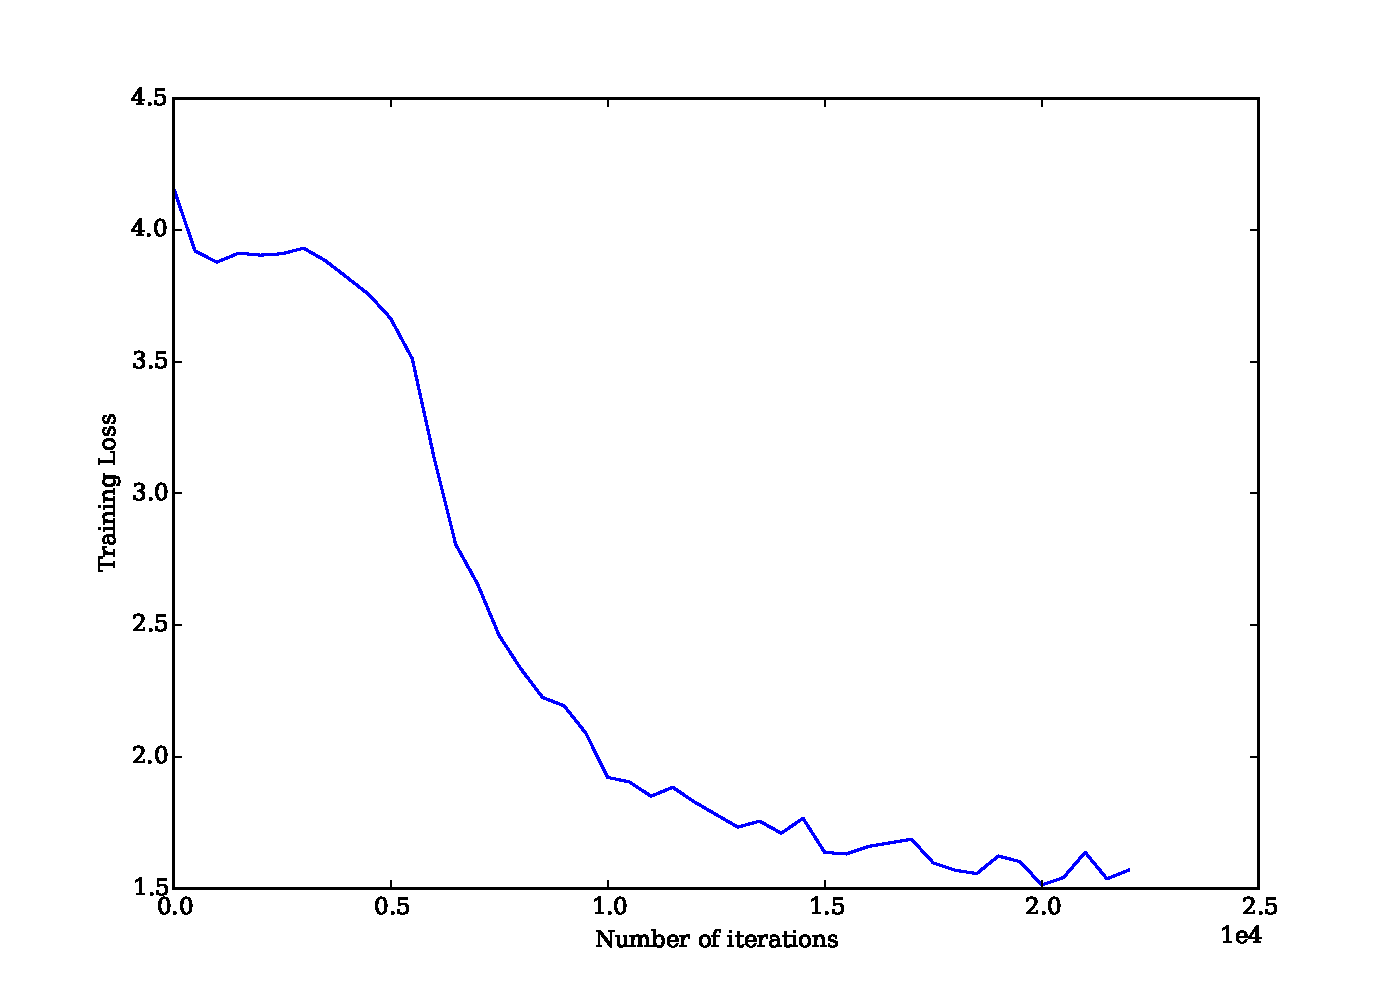
\includegraphics[width=1.0\textwidth,center]{plots/training_curve_new.pdf}
  \caption{Variation of the softmax-loss while training of 
\textsc{PIECE} model}
  \label{figure:losses}
\end{figure}
\begin{figure}
  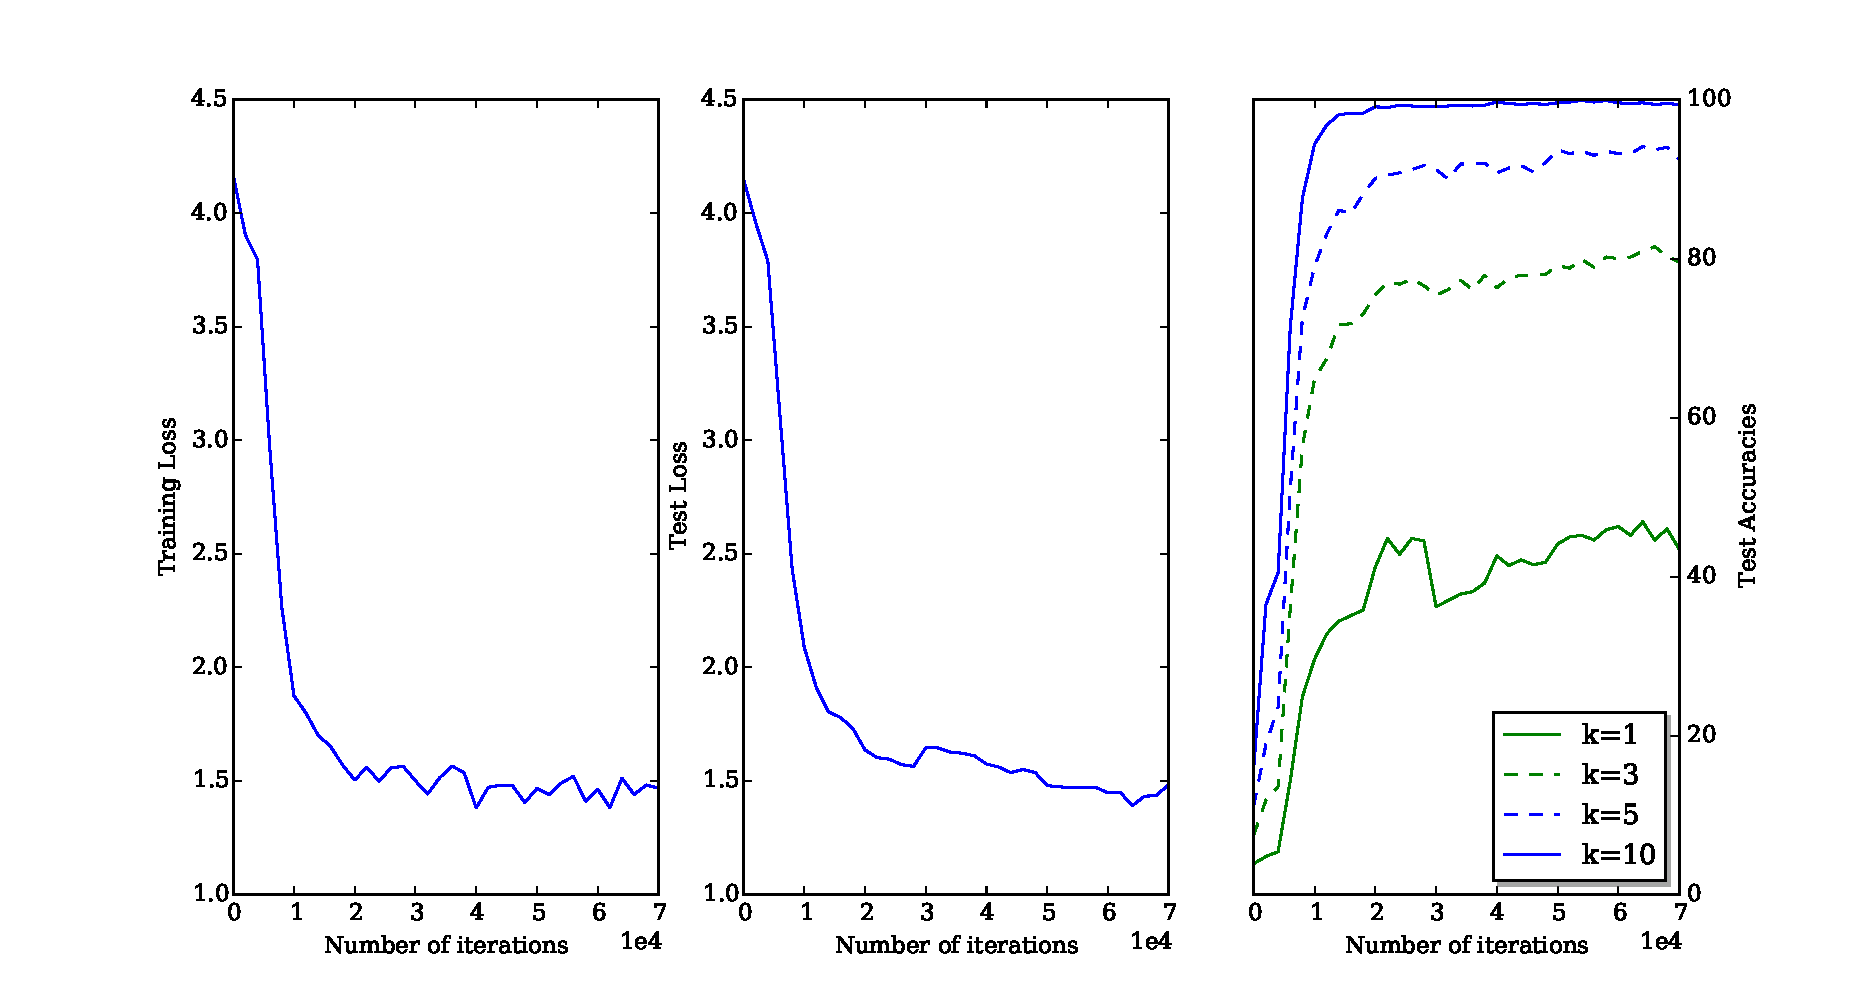
\includegraphics[width=1.55\textwidth,center]{plots/learning_curve_new.pdf}
  \caption[Variation of the accuracies on test set while training]{
  (a) Softmax-loss on training dataset (b) Softmax-loss on 
testing dataset; (c) Accuracies at k=1,3,5,10 on testing dataset.}
  \label{figure:losses-accuracies}
\end{figure}
%\section{Network Filters}

\section{Performance of \textsc{Piece} and \textsc{Move} networks}
As discussed in Chapter \ref{chap:dataset}, we divided the dataset into training 
and testing sets. We train the network, using the optimum hyper-parameters 
described in section \ref{section:hyperparams}.\\
%parameters here
The training and testing accuracies and softmax losses have been reported in the 
table below. We also report the top-k prediction accuracies for $k=3,5,10$ 
also. 
%We also compare 
% the top piece's and top move's average probability in each of the networks along 
% with the average rank of the actual move.
\begin{table}[H]
\centering
\begin{tabular}{@{}lllll@{}}
\toprule
\multirow{2}{*}{Model Name} & \multicolumn{4}{c}{Accuracy at k}                  
                                                    \\ \cmidrule(l){2-5} 
                            & \multicolumn{1}{c}{k=1} & \multicolumn{1}{c}{k=3} 
& \multicolumn{1}{c}{k=5} & \multicolumn{1}{c}{k=10} \\ \midrule
Piece                       & 56.0                    & 87.9                    
& 95.8                    & 99.5                     \\
Pawn                        & 94.8                    & 100.0                   
& 100.0                   & 100.0                    \\
Rook                        & 58.0                    & 85.2                    
& 93.5                    & 99.6                     \\
Knight                      & 77.3                    & 96.6                    
& 99.3                    & 100.0                    \\
Queen                       & 54.2                    & 81.3                    
& 90.4                    & 98.2                     \\
King                        & 71.7                    & 95.6                    
& 99.6                    & 100.0                    \\ \bottomrule
\end{tabular}
\caption{Test set performance without masking}
\label{table:performance}
\end{table}


\section{Performance after masking}
\label{sec:masking}
We hypothesize that the model will eventually learn the rules of chess through 
observation only. In this section, we will try to demonstrate how good our model 
performs in learning the rules of the game of chess.\\

Since the model has no prior information of the rules of the chess game, we can 
expect the model to make some mistakes by predicting an illegal move. For a 
legal gameplay, we use the method of \textbf{masking} the probabilities. Masking 
is done at two levels due to the inherent design of our method. First, we zero 
the probabilities of the piece positions which do not contain a friendly piece. 
Secondly, we zero out the probabilities of the final positions where the chosen 
piece type cannot reach using a single valid move.\\

After masking the probabilities for each of the board positions, we compare 
our results with the unmasked predictions to demonstrate how well our model 
has learnt the rules of chess.

\subsection{Rule learning and move legality}
We discussed how injection of chess knowledge into predicted probabilities can 
ensure that we obtain legal moves while playing. However, we also 
hypothesized that the model eventually learns the rules of the game. We will 
demonstrate this further by comparing the probability distributions obtained 
before and after masking. We use two measures to calculate the similarity 
between two distributions-- Chebyshev similarity and squared euclidean 
distance. The 
distance metrics are computed using the following expression:
\[D_{sqeuc}(p,q) = ||p-q||^2\]
\[D_{chebyshev}(p,q) = \max_{i}|p_i-q_i|\]
Both the measures are symmetric. Chebyshev distance is intuitively the maximum 
zeroed out probability value from the unmasked distribution, while the 
euclidean distance is a common measure to estimate the distance between the two 
probability vectors in the n-dimensional space (n=64 in our case). We didn't 
use KL-divergence, which is the most common measure to compute dissimilarity 
between probability distributions, since we have zero probabilities.\\

We run our experiments on a relatively small dataset of 314,740 boards and 
report the average squared euclidean distance, average Chebyshev distance 
between masked 
and unmasked probability distributions and the average number of illegal 
predictions in the table below.
\begin{table}[H]
\centering
\begin{tabular}{@{}llllll@{}}
\toprule
{\bf } & $||p-q||^2$ & $\max_i |p_i-q_i|$& Illegal move& 
\multicolumn{2}{l}{Avg Rank of actual move} \\ \cmidrule(l){5-6} 
{\bf Model}           &        &             &\%age                        & 
unmasked          & masked          \\ \midrule
{\sc Piece}  &     $3.09\times 10^{-8}$ & $4.28\times 10^{-5}$                 
    & 0.0 &2.06342060113 &2.06341424668                   
\\
{\sc Pawn}   &     $1.72\times 10^{-4}$               & $5.82\times 10^{-4}$    
                  & 0.0045 &       1.08001395504 &1.07996844947             
\\
{\sc Rook}   &             $3.74\times 10^{-3}$& $1.37\times 10^{-2}$           
 &   0.72       &2.31513493742 &2.28972185557           
\\
{\sc Knight} &       $1.74\times 10^{-5}$             &     $4.8\times 
10^{-4}$                  &       0.0 & 1.44417866616 &1.44410761652            
  
\\
{\sc Bishop}  &    $3.94\times 10^{-3}$                &  $1.15\times 10^{-2}$  
 
& 0.47                 &  1.83962121376 & 1.82638963959         
\\
{\sc Queen}  &     $5.49\times 10^{-3}$               & $1.89\times 10^{-2}$ &  
   1.23                &                   2.52614094756 &2.47512457486  
\\
{\sc King}   &    $3.35\times 10^{-3}$                &   $3.82\times 10^{-3}$ 
&       0.33            &      1.59097552371 & 1.5873805164        
\\ \bottomrule
\end{tabular}
\caption{Rule Learning}
\small\justifying
Distances between predicted probabilities and average 
percentage of illegal predictions
\label{table:rule-learning}
\end{table}
\begin{table}[H]
\centering
\begin{tabular}{@{}lll@{}}
\toprule
\multirow{2}{*}{Model} & \multicolumn{2}{l}{Percentage Accuracy} \\ 
\cmidrule(l){2-3} 
                       & before masking      & after masking     \\ \midrule
Piece                  & 56.11               & 56.11             \\
Pawn                   & 53.60               & 53.60             \\
Rook                   & 50.98               & 51.26             \\
Knight                 & 72.77               & 72.77             \\
Bishop                 & 59.89               & 60.13             \\
Queen                  & 47.99               & 48.42             \\
King                   & 64.49               & 64.76             \\ 
\bottomrule
\end{tabular}
\caption{Rule Learning: Accuracies before and after masking.}
\small\justifying
In the table above, the accuracies of each of the models is compared before 
and after masking for the set of $314,740$ board positions.
\label{table:rule-learning-2}
\end{table}

In the tables~\ref{table:rule-learning} and ~\ref{table:rule-learning-2}, we 
noticed that the models predict a legal move almost every single time when we 
are not masking the probability distributions for legal moves. This is a very 
strong result since one of the hypothesis of our work was whether the dynamics 
of chess are caused by the interactions of the pieces and the patterns they 
exist in. The convolutional neural network based models, which have no prior 
knowledge of the game of chess, can predict a legal move every single time after 
a few tens of  million games where only one in every $10^{36}$ board 
configurations has the exposed to the network. Conclusively, we can say that the 
networks which are trained on move optimality also optimize move legality, 
probably because of their extreme representation power.\\

\subsection{Evaluating performance of full move prediction}
Till now we evaluated our networks individually for piece and move prediction 
tasks. Now, we need evaluate our models in an ensembled fashion to predict the 
entire move, i.e. from and to position on the board. For this task, we evaluate 
predictions for each move as the games in our test dataset proceed. The 
plot in figure~\ref{figure:gameplay1} shows the variation of accuracy of the 
correct move (piece and destination position combined) lying in top-k 
predictions (k=1,5,10,20,30) with the index of the move into the game. The plot 
in figure~\ref{figure:gameplay2} shows the variation of mean accuracy for the 
correct move to lie in the top-k predictions (k is on the x-axis). The moves 
were predicted using the algorithm described in~\ref{alg:topprob}.
\vspace*{-1.5in}
\begin{figure}[H]
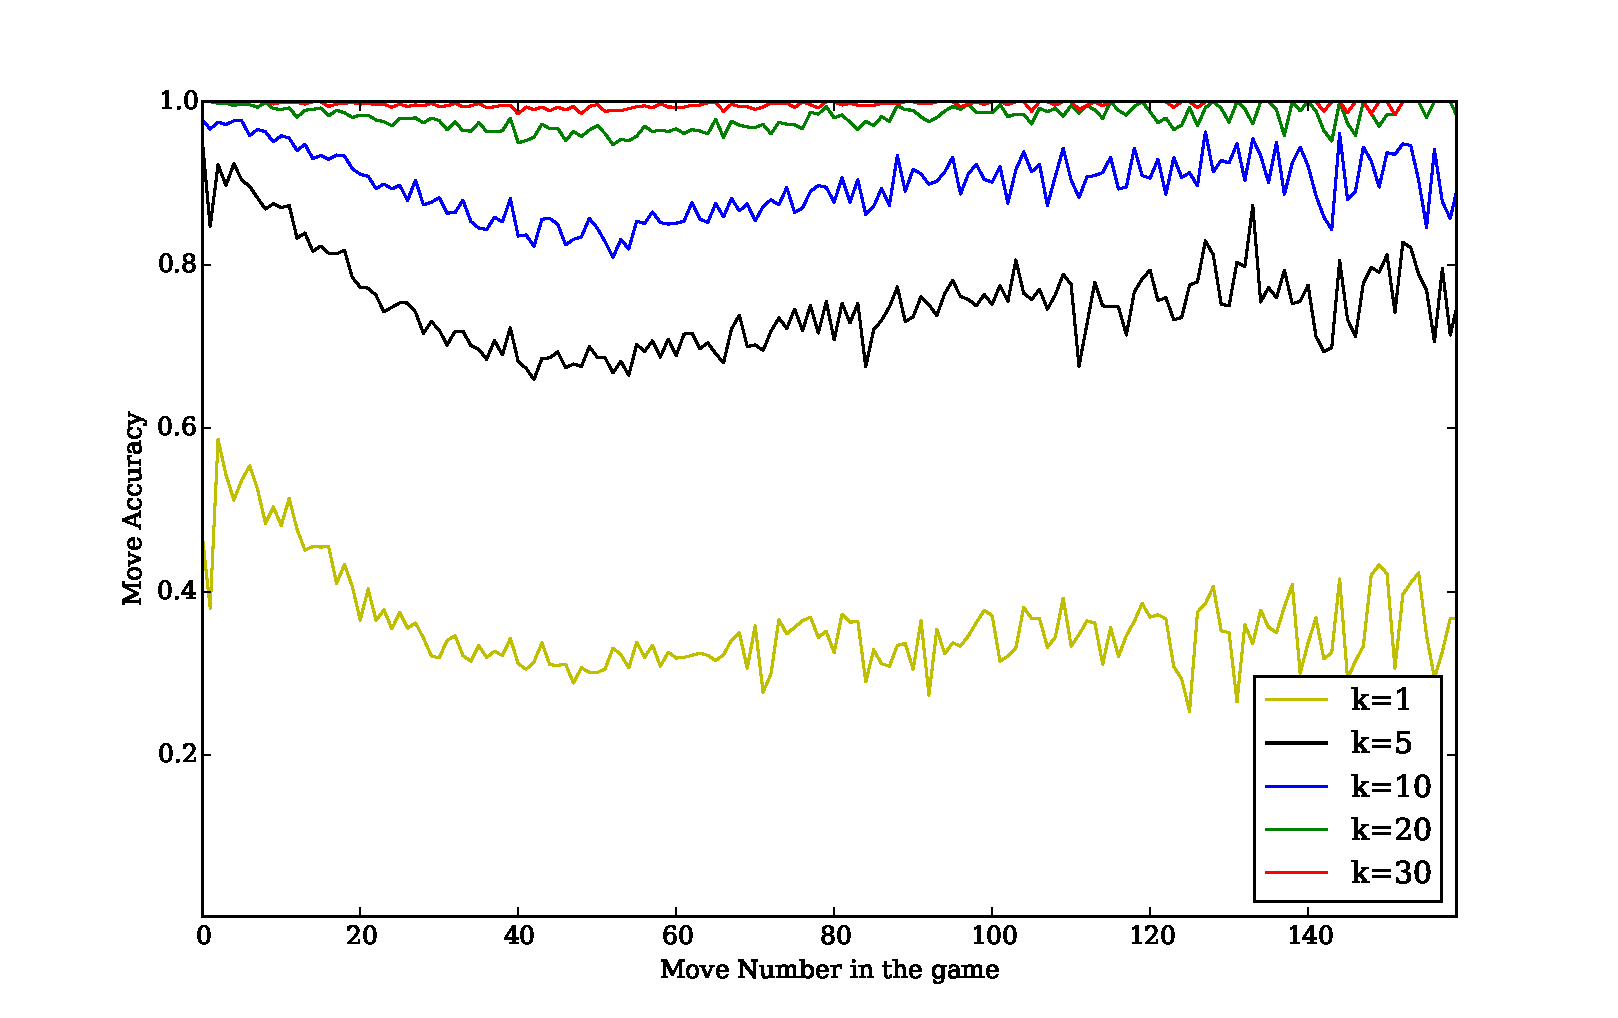
\includegraphics[width=1.3\textwidth,center]{plots/accuracy_new.pdf}
\caption[Variation of accuracies with move number]{Average accuracies at 
different move numbers in test dataset games for top k 
predictions (k=1,5,10,30).}
\label{figure:gameplay1}
\end{figure}
% \begin{figure}
% 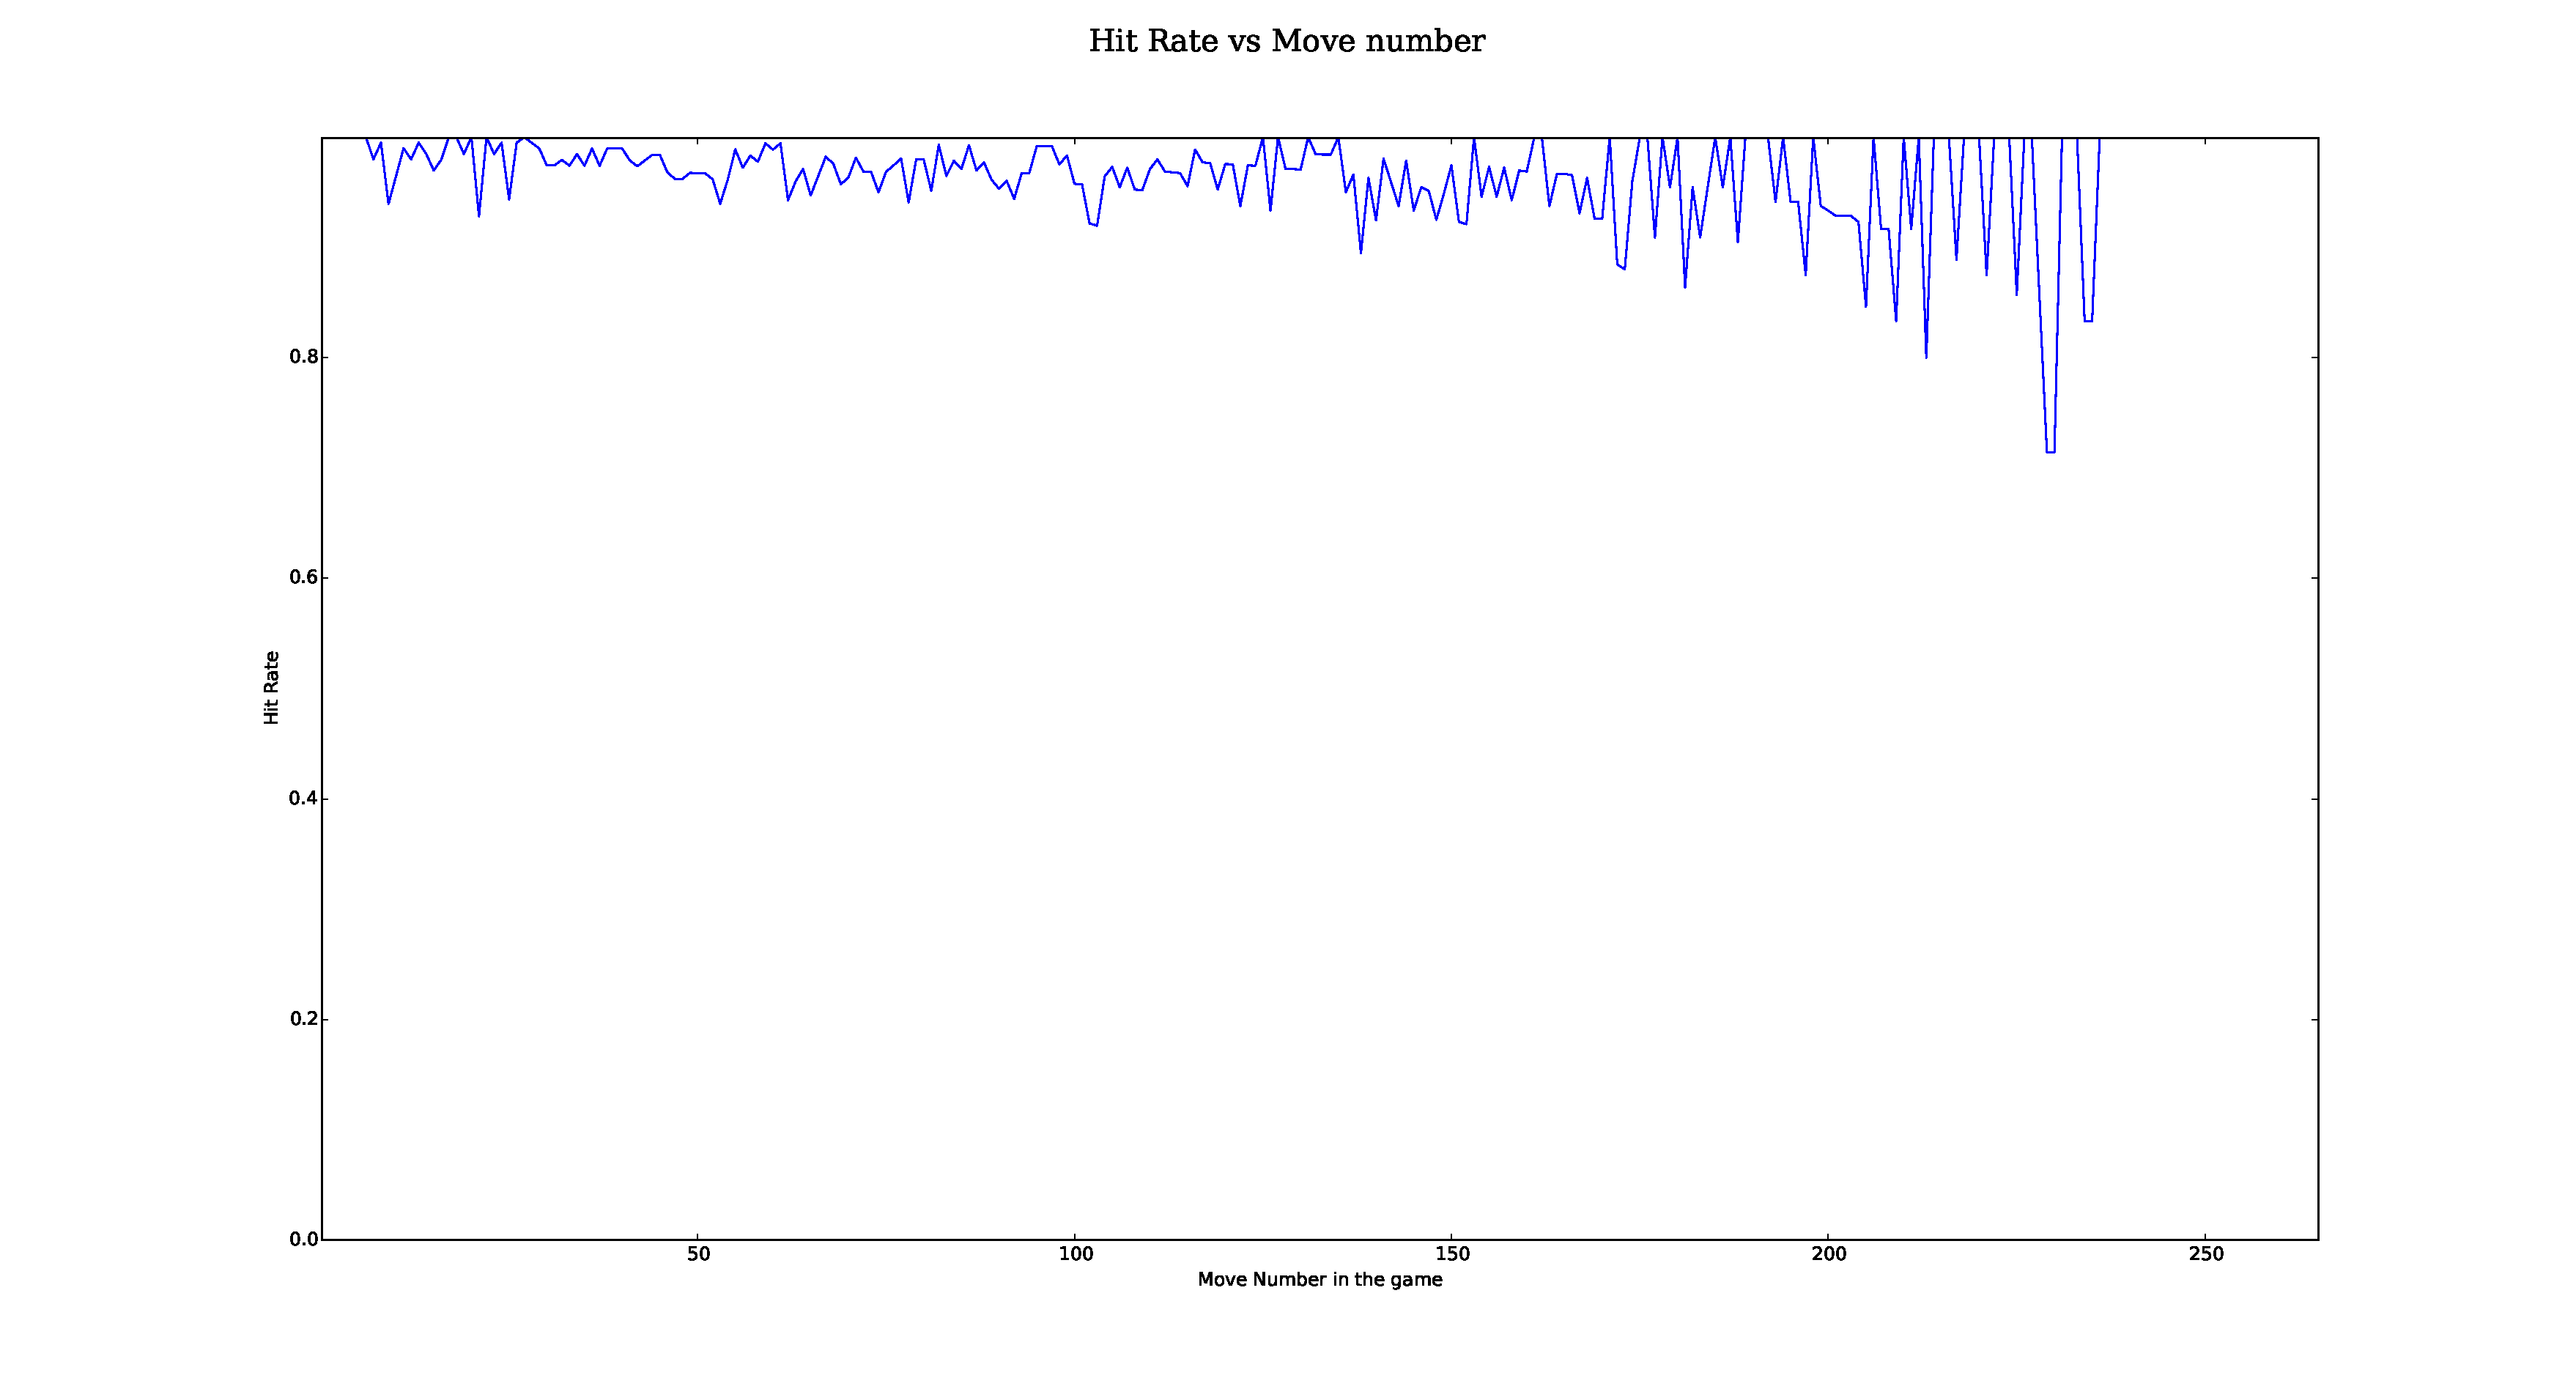
\includegraphics[width=1.5\textwidth,center]{plots/hitrate.pdf}
% \caption{Legal Move rate vs Move Number}
% \label{figure:gameplay2}
% \end{figure}
%\vspace*{-1.0in}
\begin{figure}[H]
  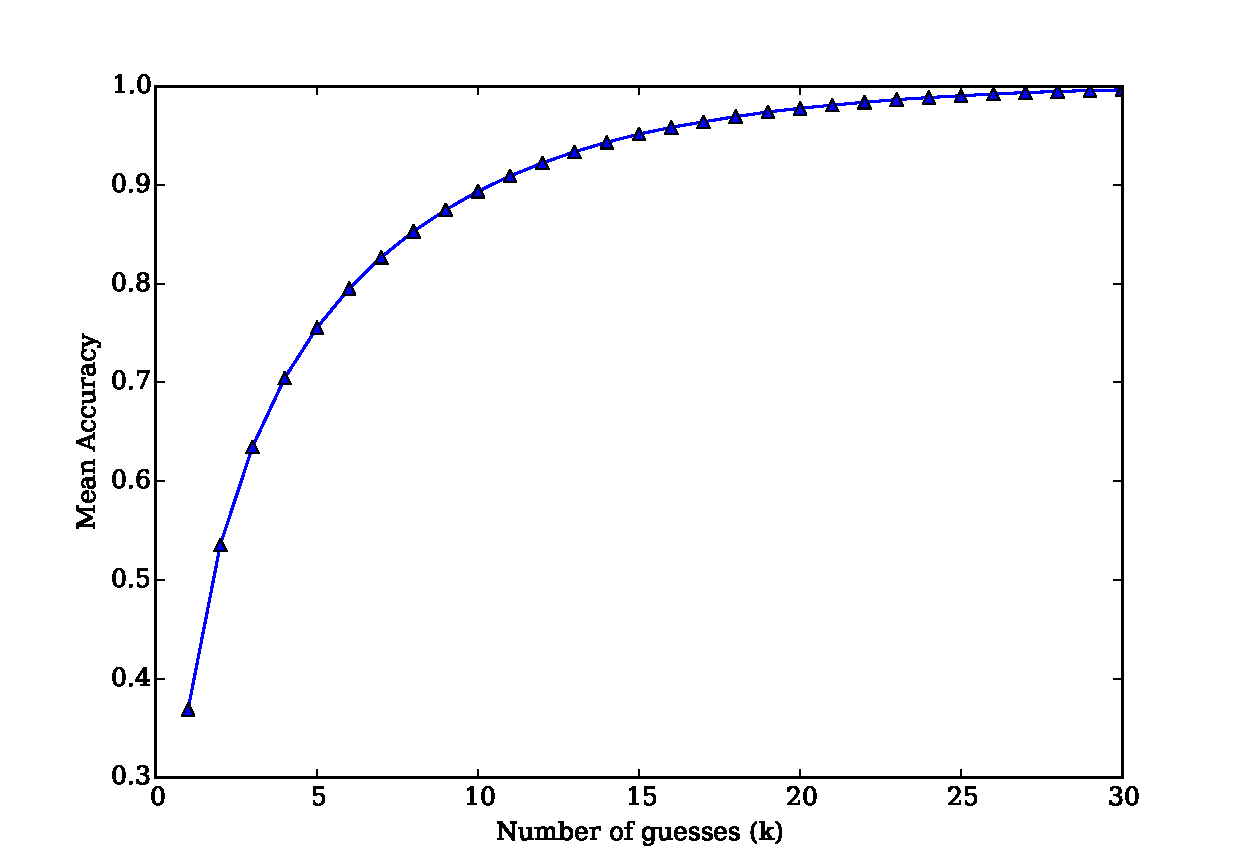
\includegraphics[width=1.0\textwidth,center]{plots/accuracy2_new.pdf}
  \caption[Variation of Top-k accuracy with k]{
  Plot of the variation of mean accuracy of the actual move lying in the 
top-k predictions with k (the number of guesses).}
  \label{figure:gameplay2}
\end{figure}
As we increase $k$ from 1 to 30, the error diminishes to less than 1\%. This 
means 1 in every hundred moves doesn't lie in top 30 of our predictions. We 
suspect that the error is caused, mostly in the middle game when a large number 
of moves are possible and the actual move played is a tactical one with a long 
term strategy in mind.
%XXX how significant is this error

\section{Sample moves taken by the network}
\label{section:samplemoves}

Here are a sample of moves predicted by the network for the board positions. We 
present two cases where the model was asked to predict the probability 
distributions for the ``from'' positions and ``to'' positions for some of the 
pieces on the board. In all the figures below, the chess board used as an input 
to the piece and move predictors. The 64-sized probability distributions are 
visualized as $8\times 8$ matrices with a color bar on the right of each. The 
probability values shown in the move selector distribution are the joint 
probabilities of piece and move selection for that specific move. 
\subsection{Initial board position}
% \vspace*{-0.5in}
We evaluate our piece and network predictors on the initial board position of a 
chess game. Figure~\ref{figure:initialboarda} shows the board position. 
Figure~\ref{figure:initialboardb} shows the distribution of the 
probabilities for the piece to be moved. Note that only the pieces in the second 
rank and the knights in the last rank can move which is apparent in the 
predictions. Table~\ref{table:initialboard} shows the comparison of the 
predicted probabilities and the percentage times the opening move was played in 
the dataset. Bobby Fischer said: ``Best by test: 1.e4'', and we shall 
see this.

\begin{figure}[H]
  \centering
    \begin{subfigure}[t]{0.5\textwidth}
        \centering
        
	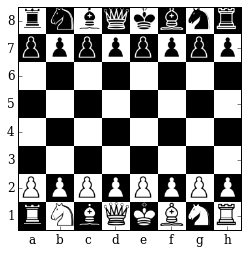
\includegraphics[scale=0.7]{img/best_moves/output_17_0.png}
        \caption{Board position(B)}
        \label{figure:initialboarda}
    \end{subfigure}%
  ~
    \begin{subfigure}[t]{0.5\textwidth}
        \centering
        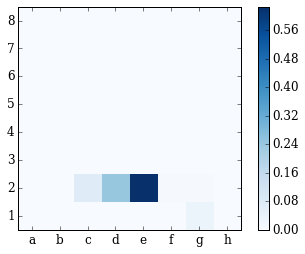
\includegraphics[width=\textwidth]{img/best_moves/output_12_0.png}
        \caption{$P_{\textsc{piece}}(B)$}
        \label{figure:initialboardb}
%         Predicted probability distribution\\
%         for the ``from'' position\\
%         predicted by \textsc{PIECE} network}
    \end{subfigure}
\caption[Predictions for initial board position]{
    (a) The initial board position for a chess game, 
    (b) The predicted probability distribution for the ``from'' piece by the 
\textsc{PIECE} network}
\label{figure:initialboard}
\end{figure}
% Please add the following required packages to your document preamble:
% \usepackage{booktabs}
\begin{table}[]
\centering
\begin{tabular}{@{}llll@{}}
\toprule
Move & Predicted Probability & Number of times played & \%age times played \\ 
\midrule
All  & 1.0000000             & 4970725                & 100.00\%           \\ 
\midrule
e2e4 & 0.6088475             & 2221439                & 44.7\%             \\
d2d4 & 0.2467637             & 1618291                & 32.6\%             \\
c2c4 & 0.0725896             & 286295                 & 5.8\%              \\
g1f3 & 0.0334573             & 334741                 & 6.7\%              \\
e2e3 & 0.0171652             & 62744                  & 1.3\%              \\
f2f4 & 0.0059381             & 67248                  & 1.4\%              \\
g2g3 & 0.0052637             & 93072                  & 1.9\%              \\
b1c3 & 0.0021147             & 98306                  & 2\%                \\
b2b3 & 0.0013837             & 64692                  & 1.3\%              \\
c2c3 & 0.0013727             & 17449                  & 0.4\%              \\
d2d3 & 0.0011852             & 43647                  & 0.9\%              \\
g2g4 & 0.0008549             & 11245                  & 0.2\%              \\
h2h3 & 0.0007792             & 5814                   & 0.1\%              \\
b2b4 & 0.0007009             & 13761                  & 0.3\%              \\
a2a3 & 0.0005240             & 5843                   & 0.1\%              \\
g1h3 & 0.0002781             & 3875                   & 0.1\%              \\
b1a3 & 0.0002716             & 1013                   & 0\%                \\
h2h4 & 0.0002087             & 7216                   & 0.1\%              \\
a2a4 & 0.0002071             & 4967                   & 0.1\%              \\
f2f3 & 0.0000310             & 9067                   & 0.2\%              \\ 
\bottomrule
\end{tabular}
\caption[Moves generated for initial board position]{Opening Move: The table 
shows the the 
moves predicted by the model alongside the predicted probability. The next two 
columns show the number of times and the percentage of times a certain opening 
was played according the the opening database on 
\url{http://www.ficsgames.org/openings.html}. The table is sorted on 
the probability predicted by our pair of networks.}
\label{table:initialboard}
\end{table}
%     ~
%   \centering
%     \begin{subfigure}[t]{0.5\textwidth}
%         \centering
%         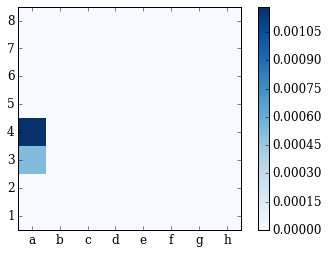
\includegraphics[width=\textwidth]{img/best_moves/output_14_0.png}
%         \caption{$P_{\textsc{pawn}}(B, a_2)$}
%         \label{figure:initialboardc}
% %         {Predicted probability distribution\\
% %         for the ``to'' position\\
% %         for a2 pawn.}
%     \end{subfigure}%
%     ~ 
%     \begin{subfigure}[t]{0.5\textwidth}
%         \centering
%         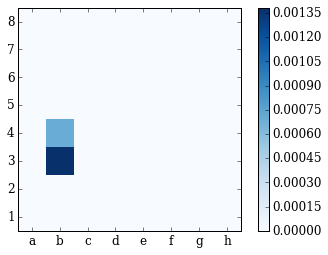
\includegraphics[width=\textwidth]{img/best_moves/output_14_1.png}
%         \caption{$P_{\textsc{pawn}}(B, b_2)$}
% %         \caption{Predicted probability distribution\\
% %         for the ``to'' position\\
% %         for b2 pawn.}
%     \end{subfigure}
%     ~
%     \begin{subfigure}[t]{0.5\textwidth}
%         \centering
%         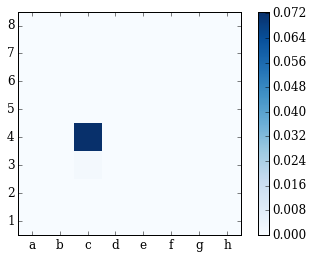
\includegraphics[width=\textwidth]{img/best_moves/output_14_2.png}
%         \caption{$P_{\textsc{pawn}}(B, c_2)$}
% %         \caption{Predicted probability distribution\\
% %         for the ``to'' position\\
% %         for c2 pawn.}
%     \end{subfigure}%
%     ~
%     \begin{subfigure}[t]{0.5\textwidth}
%         \centering
%         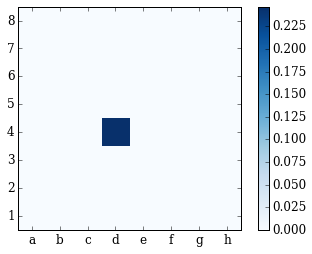
\includegraphics[width=\textwidth]{img/best_moves/output_14_3.png}
%         \caption{$P_{\textsc{pawn}}(B, d_2)$}
% %         \caption{Predicted probability distribution\\
% %         for the ``to'' position\\
% %         for d2 pawn.}
%     \end{subfigure}
% \end{figure}
% \begin{figure}[H]
%   \ContinuedFloat
%     \begin{subfigure}[t]{0.5\textwidth}
%         \centering
%         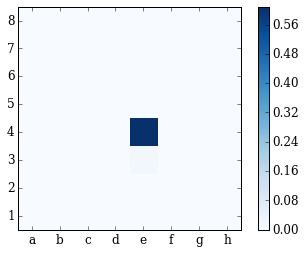
\includegraphics[width=\textwidth]{img/best_moves/output_14_4.png}
%         \caption{$P_{\textsc{pawn}}(B, e_2)$}
%     \end{subfigure}%
%     ~ 
%     \begin{subfigure}[t]{0.5\textwidth}
%         \centering
%         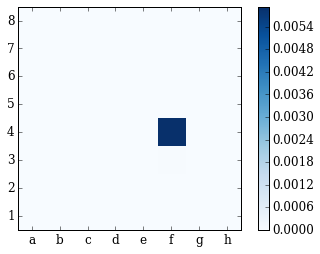
\includegraphics[width=\textwidth]{img/best_moves/output_14_5.png}
%         \caption{$P_{\textsc{pawn}}(B, f_2)$}
%     \end{subfigure}
%   ~
%     \centering
%     \begin{subfigure}[t]{0.5\textwidth}
%         \centering
%         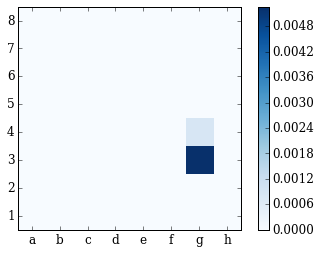
\includegraphics[width=\textwidth]{img/best_moves/output_14_6.png}
%         \caption{$P_{\textsc{pawn}}(B, g_2)$}
%     \end{subfigure}%
%     ~ 
%     \begin{subfigure}[t]{0.5\textwidth}
%         \centering
%         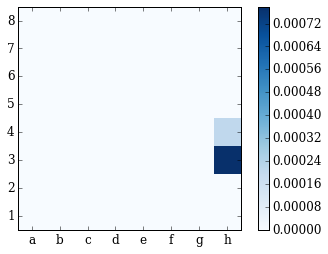
\includegraphics[width=\textwidth]{img/best_moves/output_14_7.png}
%         \caption{$P_{\textsc{pawn}}(B, h_2)$}
%     \end{subfigure}
%     ~
%     \begin{subfigure}[t]{0.5\textwidth}
%         \centering
%         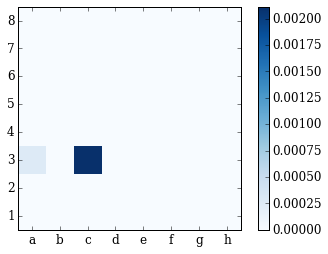
\includegraphics[width=\textwidth]{img/best_moves/output_14_8.png}
%         \caption{$P_{\textsc{knight}}(B, b_1)$}
%     \end{subfigure}%
%     ~ 
%     \begin{subfigure}[t]{0.5\textwidth}
%         \centering
%         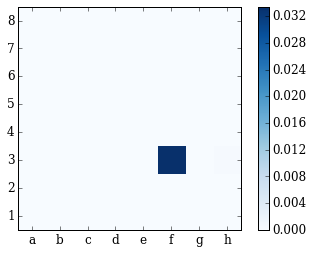
\includegraphics[width=\textwidth]{img/best_moves/output_14_9.png}
%         \caption{$P_{\textsc{knight}}(B, g_1)$}
%         \label{figure:initialboardl}
%     \end{subfigure}
%     \caption[Predictions for initial board position]{
%     (a) The initial board position for a chess game, 
%     (b) The predicted probability distribution for the ``from'' piece by the 
% \textsc{PIECE} network, 
%     (c)-(j) The predicted probability distributions for the ``to'' position by 
% the \textsc{PAWN} network for a2 to h2, 
%     (k)-(l) The predicted probability distribution for the ``to'' position by 
% the \textsc{KNIGHT} network for b1 and g1 respectively.}
% \label{figure:initialboard}
% \end{figure}


\subsection{Checkmating}
In figure \ref{figure:checkmating}, there is a checkmate possible in one move. 
We observe that the most probable move output by our model actually wins it for 
the white player.
\begin{figure}[H]
\hspace*{-0.5in}  
  \centering
    \begin{subfigure}[t]{\textwidth}
        \centering
        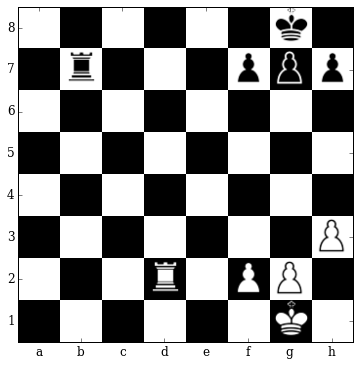
\includegraphics[scale=0.75]{img/best_moves/output_21_0.png}
        \caption{Board position. There is a check and mate 
possible in one move of the white.}
    \end{subfigure}%

 \hspace*{-0.5in}  
    \begin{subfigure}[t]{0.5\textwidth}
        \centering
        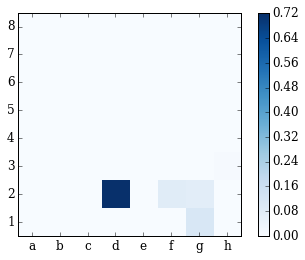
\includegraphics[width=\textwidth]{img/best_moves/output_21_2.png}
        \caption{$P_{\textsc{piece}}(B)$}
    \end{subfigure}
    ~
    \begin{subfigure}[t]{0.5\textwidth}
        \centering
        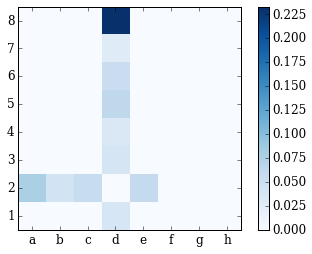
\includegraphics[width=\textwidth]{img/best_moves/output_21_6.png}
        \caption{$P_{\textsc{rook}}(B, d2)$}
    \end{subfigure}%
    \caption{Predictions for a checkmate-in-1 position}
\small
\justifying
(a) Black king is trapped in the last row. Moving the white rook 
at d2 to d8 will win the game for white. (b) The \textsc{PIECE} network 
predicts moving the rook at d2 with $p=0.72$. (c) The \textsc{ROOK} network 
predicts moving the rook to d8 with a total probability of $p=0.225$.

\label{figure:checkmating}
\end{figure}

\subsection{Detecting a check and blocking a promotion}
In figure \ref{figure:check-detection}, the king is under attack by the pawn, 
which is also seeking a promotion in the next move if the king moves away. The 
model successfully that the king should prevent the check by making the 
move \textbf{g1h1} which eventually also prevents the pawn promotion.

\begin{figure}[H]
\hspace*{-0.5in}  
  \centering
    \begin{subfigure}[t]{\textwidth}
        \centering
        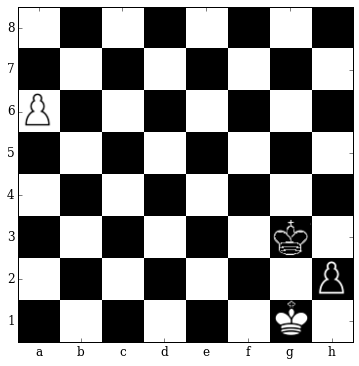
\includegraphics[scale=0.65]{img/best_moves/output_24_0.png}
        \caption{Board position. The white king is under check.}
    \end{subfigure}%

 \hspace*{-0.5in}  
    \begin{subfigure}[t]{0.5\textwidth}
        \centering
        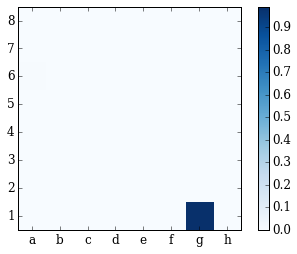
\includegraphics[width=\textwidth]{img/best_moves/output_24_2.png}
        \caption{$P_{\textsc{piece}}(B)$}
    \end{subfigure}
    ~
  \centering
    \begin{subfigure}[t]{0.5\textwidth}
        \centering
        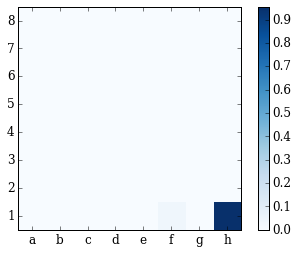
\includegraphics[width=\textwidth]{img/best_moves/output_24_6.png}
        \caption{$P_{\textsc{king}}(B, g1)$}
    \end{subfigure}%
    \caption{Prediction: Detecting a check}
    \small
    \justifying
    (a) White king is under a check. The black pawn at h2 is 
also looking for promotion in the next move. (b) The \textsc{PIECE} network 
predicts moving the king at g1 with $p>0.95$. (c) The \textsc{KING} network 
predicts moving the white king to h1 with a total probability of $p>0.9$.
\label{figure:check-detection}
\end{figure}

\subsection{En passant Move}
A very striking observation in our experiments was the the prediction of an 
en-passant move. It is interesting to note that an en-passant move is a very 
special case of  pawn movement and attack, and we might expect it to appear 
only a very few number of times in our training dataset. However, its 
effectiveness is properly captured by the ensemble of piece and move selector 
networks.
\begin{figure}[H]
\hspace*{-0.5in}  
  \centering
    \begin{subfigure}[t]{\textwidth}
        \centering
        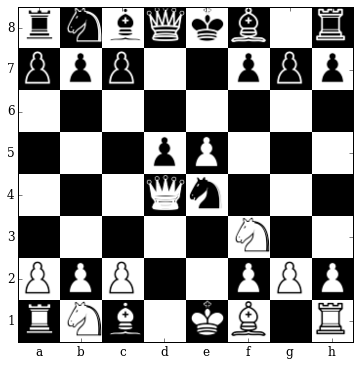
\includegraphics[scale=0.65]{img/best_moves/output_38_0.png}
        \caption{Board position. The d-pawn just moved 2 steps. En passant is 
possible}
    \end{subfigure}%

 \hspace*{-0.5in}  
    \begin{subfigure}[t]{0.5\textwidth}
        \centering
        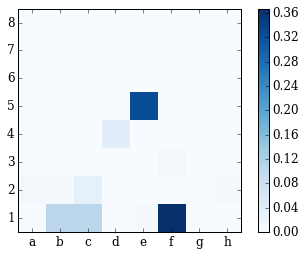
\includegraphics[width=\textwidth]{img/best_moves/output_38_2.png}
        \caption{$P_{\textsc{piece}}(B)$}
    \end{subfigure}
    ~
  \centering
    \begin{subfigure}[t]{0.5\textwidth}
        \centering
        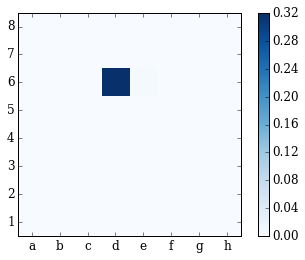
\includegraphics[width=\textwidth]{img/best_moves/output_38_6.png}
        \caption{$P_{\textsc{pawn}}(B, e5)$}
    \end{subfigure}%
    \caption{Prediction: En passant move}
    \small
    \justifying
    (a) An en-passant move is possible. (b) The maximum probable piece to move 
is the e5 pawn. (c) Unmasked probability has the en-passant move as the most 
probable move. During gameplay, if the black didn't move two steps in the last 
move, we can mask out this probability.
\label{figure:enpassant}
\end{figure}

\subsection{Castling}
In figure \ref{figure:castling} below, a castling move is predicted as the most 
favorable move.

\begin{figure}[H]
\hspace*{-0.5in}  
  \centering
    \begin{subfigure}[t]{\textwidth}
        \centering
        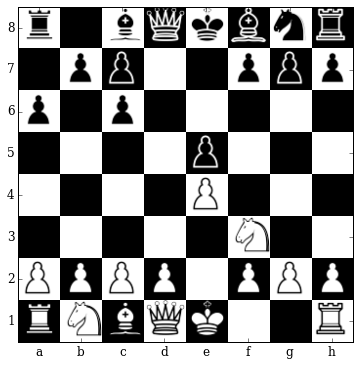
\includegraphics[scale=0.65]{img/best_moves/output_22_0.png}
        \caption{Board position. Castling is one of the favorable moves 
available.}
    \end{subfigure}%

 \hspace*{-0.5in}  
    \begin{subfigure}[t]{0.5\textwidth}
        \centering
        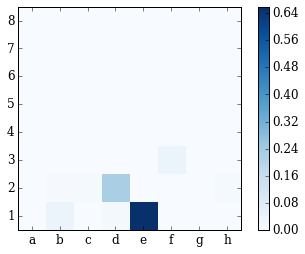
\includegraphics[width=\textwidth]{img/best_moves/output_22_2.png}
        \caption{$P_{\textsc{piece}}(B)$}
    \end{subfigure}
    ~
  \centering
    \begin{subfigure}[t]{0.5\textwidth}
        \centering
        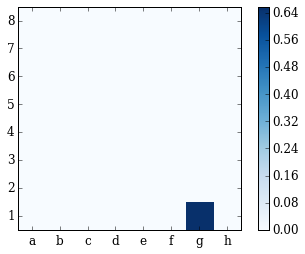
\includegraphics[width=\textwidth]{img/best_moves/output_22_6.png}
        \caption{$P_{\textsc{king}}(B, e1)$}
    \end{subfigure}%
    \caption{Prediction: Castling move}
    \small
    \justifying
    (a) Castling is available for the current board position (b) The 
\textsc{Piece} network predicts moving the king at e1 with $p>0.64$. (c) The 
\textsc{King} network predicts moving the white king to g1 with a total 
probability of $p>0.64$ completing the castling move.
\label{figure:castling}
\end{figure}

\vfill
\subsection{Middle game behavior}
Playing a move using the first guess is not ideal in a middlegame situation. 
Most of the players try to adopt tactics and long term strategies. However, our 
network trained on just 1 step outputs, may not be aware of such strategies. 
But, it is worth observing the behavior of our model when it comes to blunders 
by the opponents and we can take advantage of it.

We present here a game between Magnus Carlsen (white) and Viswanathan Anand 
(black), where Carlsen made a mistake at the 26th move while he easily had a 
good control of the game. Anand oversaw the better move Nex5! to play a4?. Anand 
later realized his mistake, but it was too late and Carlsen had already regained 
the control over the board.\\

We make our model predict the moves Vishwanathan 
Anand should have played after Carlsen's blunder. It is worth noting that the 
most favorable move as suggested by experts was Nex5 (i.e. g6e5), while Anand 
played a4 (i.e. a5a4). Our model predicts that the more favorable move be played 
with a much higher probability (around 6 times) than the actual move. Since 
it is not the best ranked move in our model's prediction, this also 
demonstrates the need to use search along with a prediction model to play a 
better game especially during the middle games. \\

The commentary is available at: \\
\url{http://en.chessbase.com/post/sochi-g6-carlsen-won-anand-missed-big-chance}
Most of the commentators following the game called Anand's move 26 a missed 
opportunity. A tweet said-- \textit{``Wow 26...Ne5! and black is 
winning....Anand plays 26...a4? Whats going on :) \#CarlsenAnand''}

\begin{figure}[H]
\hspace*{-0.5in}  
  \centering
  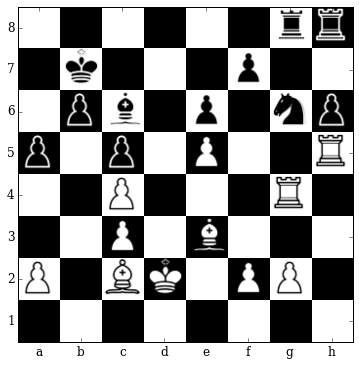
\includegraphics[scale=0.65]{img/best_moves/vishy-magnus.png}
  \caption[Middle game case study]{Black to move. 26th move. 6th game of 
the World Championship match, 2014-- Magnus Carlsen vs Viswanathan Anand}

\label{figure:carlsen-vs-vishy}
\end{figure}

\begin{table}[H]
\centering
\begin{tabular}{@{}lll@{}}
\cmidrule(r){1-2}
Move & Predicted Probability &                                  \\ 
\cmidrule(r){1-2}
g8d8 & 0.252880722284        &                                  \\
g8g7 & 0.148237019777        &                                  \\
g6e5 & 0.13111974299         & Expected Move                    \\
b7c7 & 0.0660261586308       &                                  \\
h8h7 & 0.0471959412098       &                                  \\
c6g2 & 0.0403394699097       &                                  \\
c6e8 & 0.0358173549175       &                                  \\
g8c8 & 0.0323895104229       &                                  \\
b7c8 & 0.0302288047969       &                                  \\
c6d7 & 0.0250529013574       &                                  \\
a5a4 & 0.0231475103647       & Vishwanathan Anand's actual move \\
g6e7 & 0.0229441132396       &                                  \\
b7a6 & 0.0208601523191       &                                  \\
g8a8 & 0.0198916308582       &                                  \\
b7b8 & 0.0190593209118       &                                  \\
c6a4 & 0.0153007712215       &                                  \\
g6f8 & 0.0150824002922       &                                  \\
g8f8 & 0.0115283448249       &                                  \\
g8e8 & 0.00727259740233      &                                  \\
b7a7 & 0.00666899653152      &                                  \\ 
\cmidrule(r){1-2}
\end{tabular}
\caption{Possible moves after the mistake by Carlsen in Move 26}
\label{table:vishy-carlsen}
\end{table}

\section{Board Evaluations}
\label{section:boardevaluations}
In this section we will look at some of the evaluation values 
($V_\gamma(board)$) predicted by the CNN trained to learn an evaluation 
function ($V_\gamma$) as described in chapter \ref{chap:implementation}. For 
each board position, we present boards with the highest evaluation values that 
can be reached from the current board position through a legal move. For 
probity, we also include the moves that might leave or put the king in check, 
but are otherwise valid. We also include legal castling moves.

\begin{figure}[H]
\vspace{-0.2in}
\hspace*{-0.5in}  
  \centering
    \begin{subfigure}[t]{\textwidth}
        \centering
        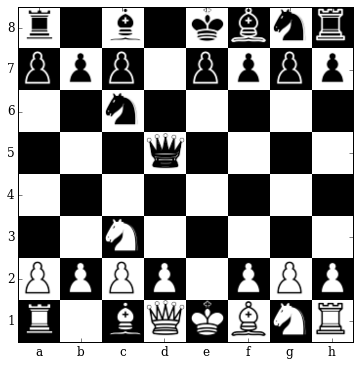
\includegraphics[scale=0.55]{img/table_evaluations/output_11_0.png}
        \caption{Board position (White to move)}
    \end{subfigure}%

 \hspace*{-0.5in}  
    \begin{subfigure}[t]{0.45\textwidth}
        \centering
        
    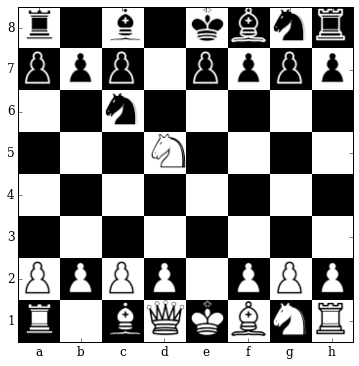
\includegraphics[width=\textwidth]{img/table_evaluations/output_11_2.png}
        \caption{Move: c3d5\\
        $V_{\gamma=0.7}=0.0545$}
    \end{subfigure}
   \hspace{1em}
  \centering
    \begin{subfigure}[t]{0.45\textwidth}
        \centering
        
    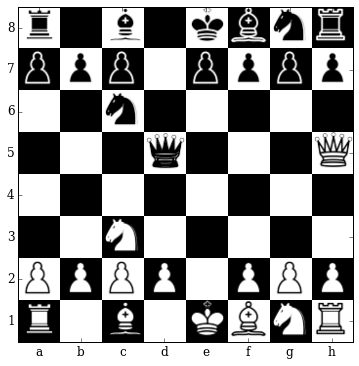
\includegraphics[width=\textwidth]{img/table_evaluations/output_11_4.png}
        \caption{Move: d1h5\\
        $V_{\gamma=0.7}=0.0144$}
    \end{subfigure}
    \caption{Evaluation function: Capturing a Queen with a knight}
    \small
    \justifying
(a) Black has made a mistake by moving the queen to an open position where 
it is under attack from a white knight; (b)-(c) The top two evaluated boards 
reachable from the current position through a legal move.
\label{figure:eval:queen-capture}
\end{figure}

\begin{figure}[H]
\vspace{-0.2in}
\hspace*{-0.5in}  
  \centering
    \begin{subfigure}[t]{\textwidth}
        \centering
        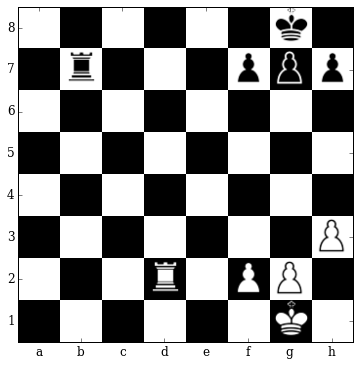
\includegraphics[scale=0.55]{img/table_evaluations/output_12_0.png}
        \caption{Board position (White to move)}
    \end{subfigure}%

 \hspace*{-0.5in}  
    \begin{subfigure}[t]{0.45\textwidth}
        \centering
        
    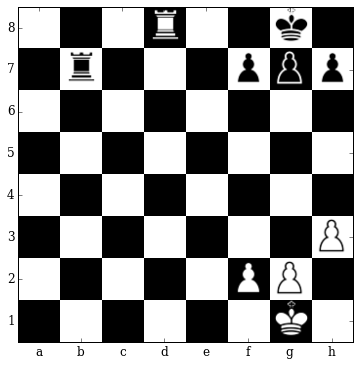
\includegraphics[width=\textwidth]{img/table_evaluations/output_12_2.png}
        \caption{Move: d2a8\\
        $V_{\gamma=0.7}=0.0543$}
    \end{subfigure}
   \hspace{1em}
  \centering
    \begin{subfigure}[t]{0.45\textwidth}
        \centering
        
    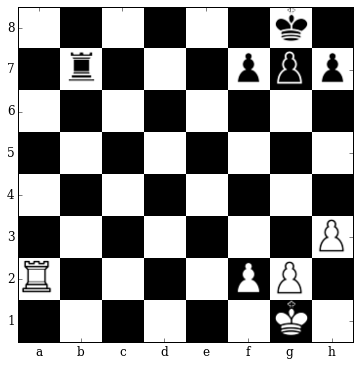
\includegraphics[width=\textwidth]{img/table_evaluations/output_12_4.png}
        \caption{Move: d2a2\\
        $V_{\gamma=0.7}=0.0177$}
    \end{subfigure}
    \caption{Evaluation function: Checkmate in one move}
    \small
    \justifying
    (a) A checkmate is possible in just one move of white; (b) The board with 
highest evaluation score in one move distance from the current board. It is a 
check and a mate. (c) The second best move predicted by the evaluation 
function. The value is less than 0.4 times the highest value.
\label{figure:eval:checkmate}
\end{figure}

\begin{figure}[H]
\vspace{-0.2in}
\hspace*{-0.5in}  
  \centering
    \begin{subfigure}[t]{\textwidth}
        \centering
        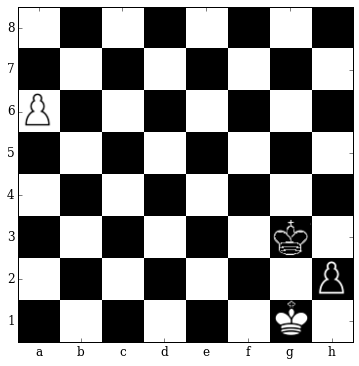
\includegraphics[scale=0.55]{img/table_evaluations/output_15_0.png}
        \caption{Board position (White to move)}
    \end{subfigure}%

 \hspace*{-0.5in}  
    \begin{subfigure}[t]{0.45\textwidth}
        \centering
        
    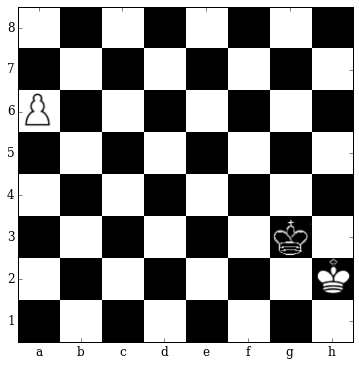
\includegraphics[width=\textwidth]{img/table_evaluations/output_15_2.png}
        \caption{Move: g1h2 \\
        $V_{\gamma=0.7}=0.0216$}
    \end{subfigure}
   \hspace{1em}
  \centering
    \begin{subfigure}[t]{0.45\textwidth}
        \centering
        
    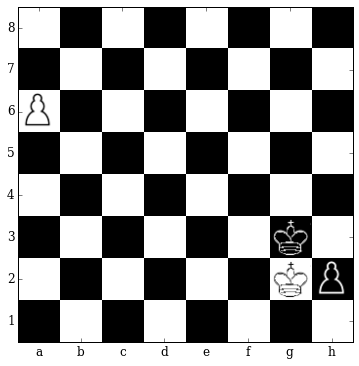
\includegraphics[width=\textwidth]{img/table_evaluations/output_15_4.png}
        \caption{Move: g1g2 \\
        $V_{\gamma=0.7}=0.0084$}
    \end{subfigure}
    \caption{Evaluation function: Check detection and promotion prevention}
    \small
    \justifying
    (a) White to move. The white king is currently under check by the black 
pawn at h2. If the king moves away, the pawn will promote to a queen and can 
wrap up the game easily afterwards; (b) The board with the highest evaluation 
is the one where the king captures the pawn. (c) The board with the second 
highest evaluation is the one where the king puts itself into check.
\label{figure:eval:check-promotion}
\end{figure}

There are a couple of interesting observations that we can make from the few 
examples above:
\begin{enumerate}
 \item \textbf{Piece Capture}
 In figures \ref{figure:eval:queen-capture} and 
\ref{figure:eval:check-promotion}, the boards with highest value in the next 
move have one less opponent piece than the preceding board i.e. a white piece 
captures a black piece. This is not the case in figure 
\ref{figure:eval:checkmate}, probably because there was no direct piece capture 
possible.
 \item \textbf{Board value is analogous to sum of piece values} In most of the 
examples above, %as well as the ones in Appendix
we can observe a similar trend-- the board is evaluated in a way similar to a 
function that computes the difference in the values of the pieces remaining for 
both the players. We will probe further into this observation further in 
\ref{subsection:correlation} where we see the correlation between this and a 
common piece evaluation system.
\end{enumerate}

\subsection{Correlation with the Material heuristic}
\label{subsection:correlation}
To investigate the properties of the evaluation function, we computed the 
correlation of the values given by $V_\gamma(board)$ with the following 
heuristically derived evaluation function ($V_{\textsc{MATERIAL}}(board)$):
\begin{table}[H]
\centering
\begin{tabular}{@{}llllll@{}}
\toprule
{\bf Piece} & Pawn & Rook & Knight  & Bishop & Queen \\ \midrule
{\bf Value} & 1    & 5    & 3	    & 3      & 9     \\ \bottomrule
\end{tabular}
\caption{The most common assignment of piece valuations}
\end{table}
Some variations value the king highly, we do not use any such assignment 
because kings are present for both the players during the whole course of the 
game and hence won't impact our evaluation as such.\\

So the function $V_{\textsc{MATERIAL}}$ is as follows:\\
$V_{\textsc{MATERIAL}}(board) = 1 \times (P-P') + 3 \times (N-N')+ 3 \times 
(B-B') + 5 
\times (R-R')+ 9 \times (Q-Q')$\\
\hspace{0.25in}where $P, N, B, R, Q$ represent the number of pawns, knights, 
bishops, rook, queen respectively for the white player and $P', N', B', R', Q'$ 
refer to their black counterparts.\\

The value of Pearson's correlation coefficient\footnote{Pearson's 
correlation coefficient ($\rho$) between two random variables is also 
referred to as the \textit{product moment} i.e. the mean of the product of the 
adjusted random variables. It can be computed using the formula: $\rho = 
\frac{E[(X-\mu_X)(Y-\mu_Y)]}{\sigma_X\sigma_Y}$
} we obtain for a set of $665,727$ boards between evaluation done with the 
model 
$V_{\gamma=0.7}$ and $V_{\textsc{MATERIAL}}$ is \textbf{0.8194}. 
Figure~\ref{figure:correlation} plots the evaluation function values for two 
functions 
for different boards. The correlation seems evident from the scatter plot. We 
also consider some example boards in figure~\ref{figure:correlation2}. The 
boards with a positive material value for white have a positive evaluation in 
our function. It is worth noting that in figure~\ref{figure:correlation2d}, 
white has almost won and it has a board value of 20 and an evaluation function 
suggests that white is approximately 3 moves away from winning ($(0.7)^3 = 
0.34$).\\

\begin{figure}[H]
 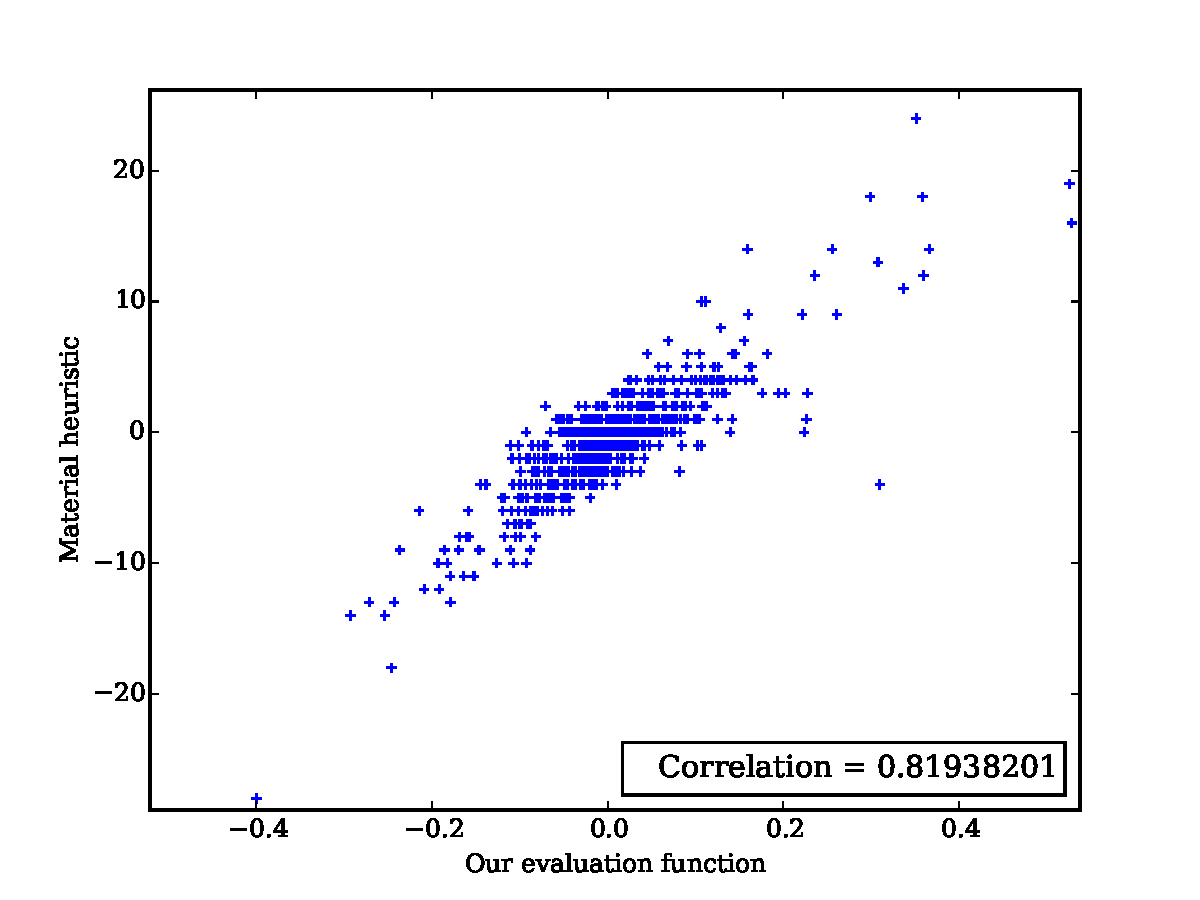
\includegraphics[scale=0.75]{plots/correlation_eval.pdf}
 \caption[Correlation between $V_{\gamma=0.7}$ and 
$V_{\textsc{MATERIAL}}$]{Scatter plot showing $V_{\gamma=0.7}$ and 
$V_{\textsc{MATERIAL}}$ values for different boards in the test dataset}
\label{figure:correlation}
\end{figure}

\begin{figure}[h]
\vspace{-0.2in}
\hspace*{-0.5in}  
  \centering
    \begin{subfigure}[t]{0.45\textwidth}
        \centering
        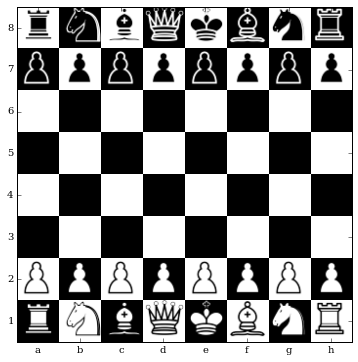
\includegraphics[scale=0.55]{img/table_evaluations/output_35_0.png}
        \centering
        \caption{$V_{\gamma=0.7} = 0.0015796$\\  
$V_{\textsc{MATERIAL}}= 0.0 $}
  \label{figure:correlation2d}
    \end{subfigure}%
    \hspace{1em}
    \begin{subfigure}[t]{0.45\textwidth}
        \centering
        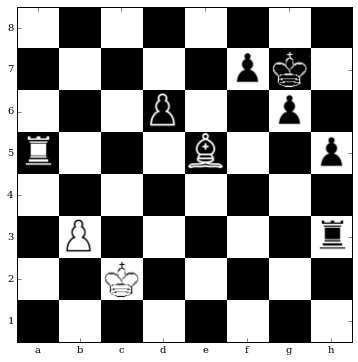
\includegraphics[scale=0.55]{img/table_evaluations/output_33_0.png}
         \caption{$V_{\gamma=0.7} = -0.0748723$\\  
$V_{\textsc{MATERIAL}}= -6.0 $}
    \end{subfigure}%

 \hspace*{-0.5in}  
    \begin{subfigure}[t]{0.45\textwidth}
        \centering
        
    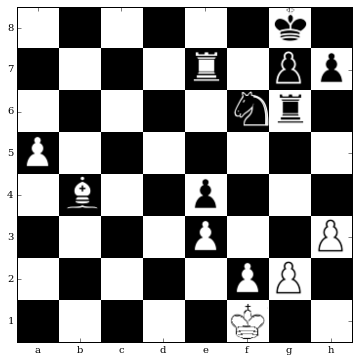
\includegraphics[width=\textwidth]{img/table_evaluations/output_34_0.png}
         \caption{$V_{\gamma=0.7} = 0.0902274$\\  
$V_{\textsc{MATERIAL}}= 2.0 $}
    \end{subfigure}
   \hspace{1em}
  \centering
    \begin{subfigure}[t]{0.45\textwidth}
        \centering
        
    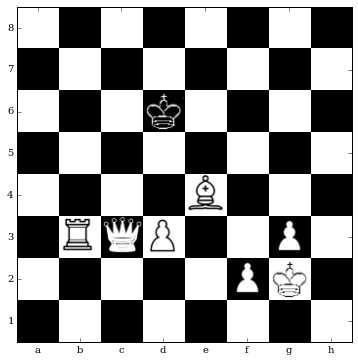
\includegraphics[width=\textwidth]{img/table_evaluations/output_36_0.png}
         \caption{$V_{\gamma=0.7} = 0.302926$\\  
$V_{\textsc{MATERIAL}}= 20.0 $}
    \label{figure:correlation2d}
    \end{subfigure}
    \caption{Comparing the evaluation functions $V_{\gamma=0.7}$ and 
$V_{\textsc{MATERIAL}}$ }
\label{figure:correlation2}
\end{figure}


While a correlation coefficient of 0.8194 is pretty impressive, it doesn't 
actually imply a good evaluation function. Rather it provides a significant 
evidence of the nature of the evaluation function learned by our CNN based 
architecture without any prior knowledge of the importance of pieces or even any 
knowledge of the rules. The difference however is that the CNN based evaluation 
function is much more complex and makes use of shared weights to score local 
patterns to evaluate the complete board. This is what motivated to solve a 
regression problem using a convolutional neural network.\\

Although there are significant variations to the basic evaluation scheme we 
compare here, like the ones that score single pieces or pairs of pieces on the 
basis of its rank and file and/or the number of liberties, we omit comparing 
our evaluation function against them since our aim was just to present a idea of 
the similarity between such a set of hand-crafted heuristically defined 
evaluation functions.

\subsection{Game Trajectories}
\begin{figure}[H]
  \hspace*{-1.0in}
 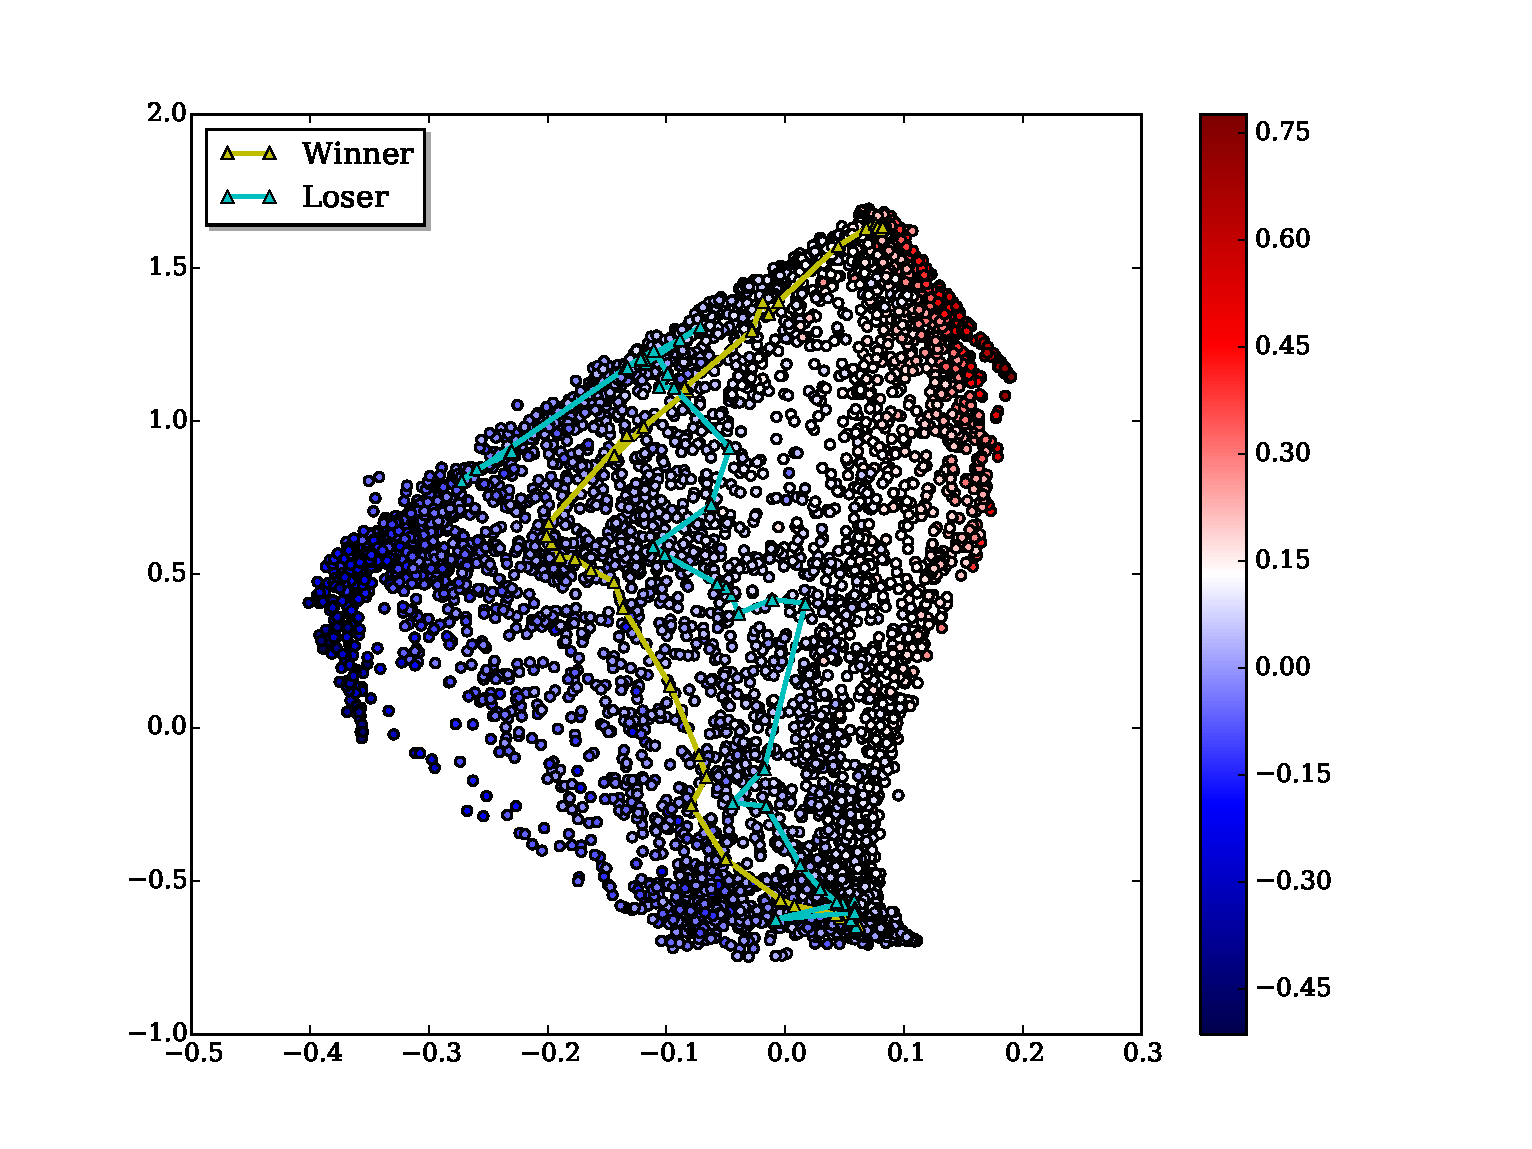
\includegraphics[width=1.5\textwidth]{plots/board_evals_win.pdf}
 \caption[Game Trajectories]{t-SNE embedding of the activations at the last 
fully connected layer of the board evaluation CNN. The red end is the set of 
boards close to winning, the blue end is the set of boards close to losing 
a game. We plot a game on the embedding. The winner(yellow) ends on the red 
side of the embedding while the loser(cyan) ends on the blue side of the 
embedding}
\end{figure}
\label{subsection:trajectories}
As an analysis to the evaluation function proposed, we tried to observe the 
evaluations of the boards observed in a few test set games. In 
figure~\ref{figure:gametrajectory}, the scatter plot shows a set of $10,000$ 
boards from our test dataset embedded onto a two dimensional embedding of 
the activations caused at the last fully connected layer of the board 
evaluation CNN using t-SNE~\cite{tsne}. The game trajectories i.e. the path of 
the boards as seen on the two dimensional embedding for both the winning and 
the losing players is shown on the plot. A description of the game could be that 
the two players had boards with similar evaluation before one of them starts to 
win i.e. gets to see boards with higher positive evaluation values.\\




\section{Gameplay}
In this section we describe and discuss how well our models do when playing 
against a computer. It needs to be emphasized again that the primary 
motivation of our work is not the build the strongest chess playing 
system, but to show as a proof of concept that the convolutional neural 
network architecture can indeed learn how to play chess and also make strong 
predictions. \\
We already demonstrated the strengths and weaknesses of both our 
models on various cases in a game of chess. Since the actual gameplay is 
tougher than solving individual cases even with high accuracy, we may expect our 
system to make blunders which makes it lose matches. It is apparent that a 
heuristic search with a large amount of chess knowledge can help make the system 
robust to blunders.\\

Since our entire source code is in \textit{Python}, we wanted to choose a 
Python based chess playing system which was easy to integrate with our 
prediction and evaluation system rather than be in an arms race with the best 
systems like Rybka \cite{wiki:rybka} and Stockfish, which use optimizations and 
tweaks upto 
the level of memory addresses and assembly code generation. We went for Sunfish 
\cite{sunfish}, which is a short and lucid python chess program which implements 
MTD-f for search. We also utilize the API like structure of Sunfish to inject 
the minimal chess knowledge required for our system and hence play the predicted 
moves.\\

\begin{table}[width=1.5\textwidth]
\centering
\hspace*{-1.0in}
\begin{tabular}{@{}llllll@{}}
\toprule
{\bf Method Used} & Games Played & Won & Drawn & Lost & 
Details                      \\ \midrule
Top-Prob          & 73           & 7         & 20          & 46         & 
$10\leq maxn\leq 1000$ \\\\
TopProb-Negamax&19     &3        &4		   & 12           & 
$10\leq maxn\leq 100$ \\\\
Evaluation function ($V_{\gamma=0.7}$)&&&&&\\
with Negamax &   21      & 6  &   4           & 11       &  2 \textless Negamax 
depth \textless 5 \\\\
Evaluation function ($V_{\gamma=0.7}$)&&&&&\\
with Negamax& 25        &  16 & 2             & 7       & Negamax depth=4       
                      \\\\
%                   &              &           &             &            &        
%                       \\
%                   &              &           &             &            &        
%                       \\
%                   &              &           &             &            &        
%                       \\ 
                      \bottomrule
\end{tabular}
\hspace*{-1.2in}
\caption[Results against negamax]{The table shows the result statistics for 
evaluation of gameplay against sunfish. We test our models under different 
conditions. In most of our experiments we limit the number of nodes explored by 
Sunfish between 10 to 1000 (chosen randomly on a log scale). For other 
deviations, the details are mentioned in the details column}
\label{table:gameplay}
\end{table}

The fact that our models do not perform well against Sunfish, that too with 
limited search capability, is not disheartening. Looking at the implementations 
of some of the best-known chess computers with all the bitmap optimizations 
and computations, we believe that there is still a long way in a Convolutional 
neural network becoming the primary backend of such a system. As we already 
emphasized enough, that the aim of our work has never been to be in an arms 
race with the best known chess computers around, but to provide a proof of 
evidence that convolutional neural networks can indeed play a game of chess.\\

It is worth mentioning that examples like the model learning to predict only 
the legal moves at any board position is a strong result in itself. Further, 
the analysis shown earlier in the chapter (sections~\ref{section:samplemoves}, 
\ref{section:boardevaluations}) shows positive outcomes for even some of the 
tricky cases. Also, during the gameplay it was observed that a proper pawn 
structure, castling move and defense for the king were prominent features of 
most of the games. This strengthens the evidence this work provides in 
human-like chess players with generalization and pattern recognition capability. 
 We discuss about these strengths, possible reasons for the weaknesses and 
propose extensions of this work in the next chapter.

% \subsection{}
% Since the individual networks have to predict from a set of size 64, the 
% evaluation cannot be made with respect to the actual move which comes from a 
% set of $64\times 64$. Hence, we evaluate predictions as the games in our test 
% dataset proceed.  
% 
% \begin{figure}
% 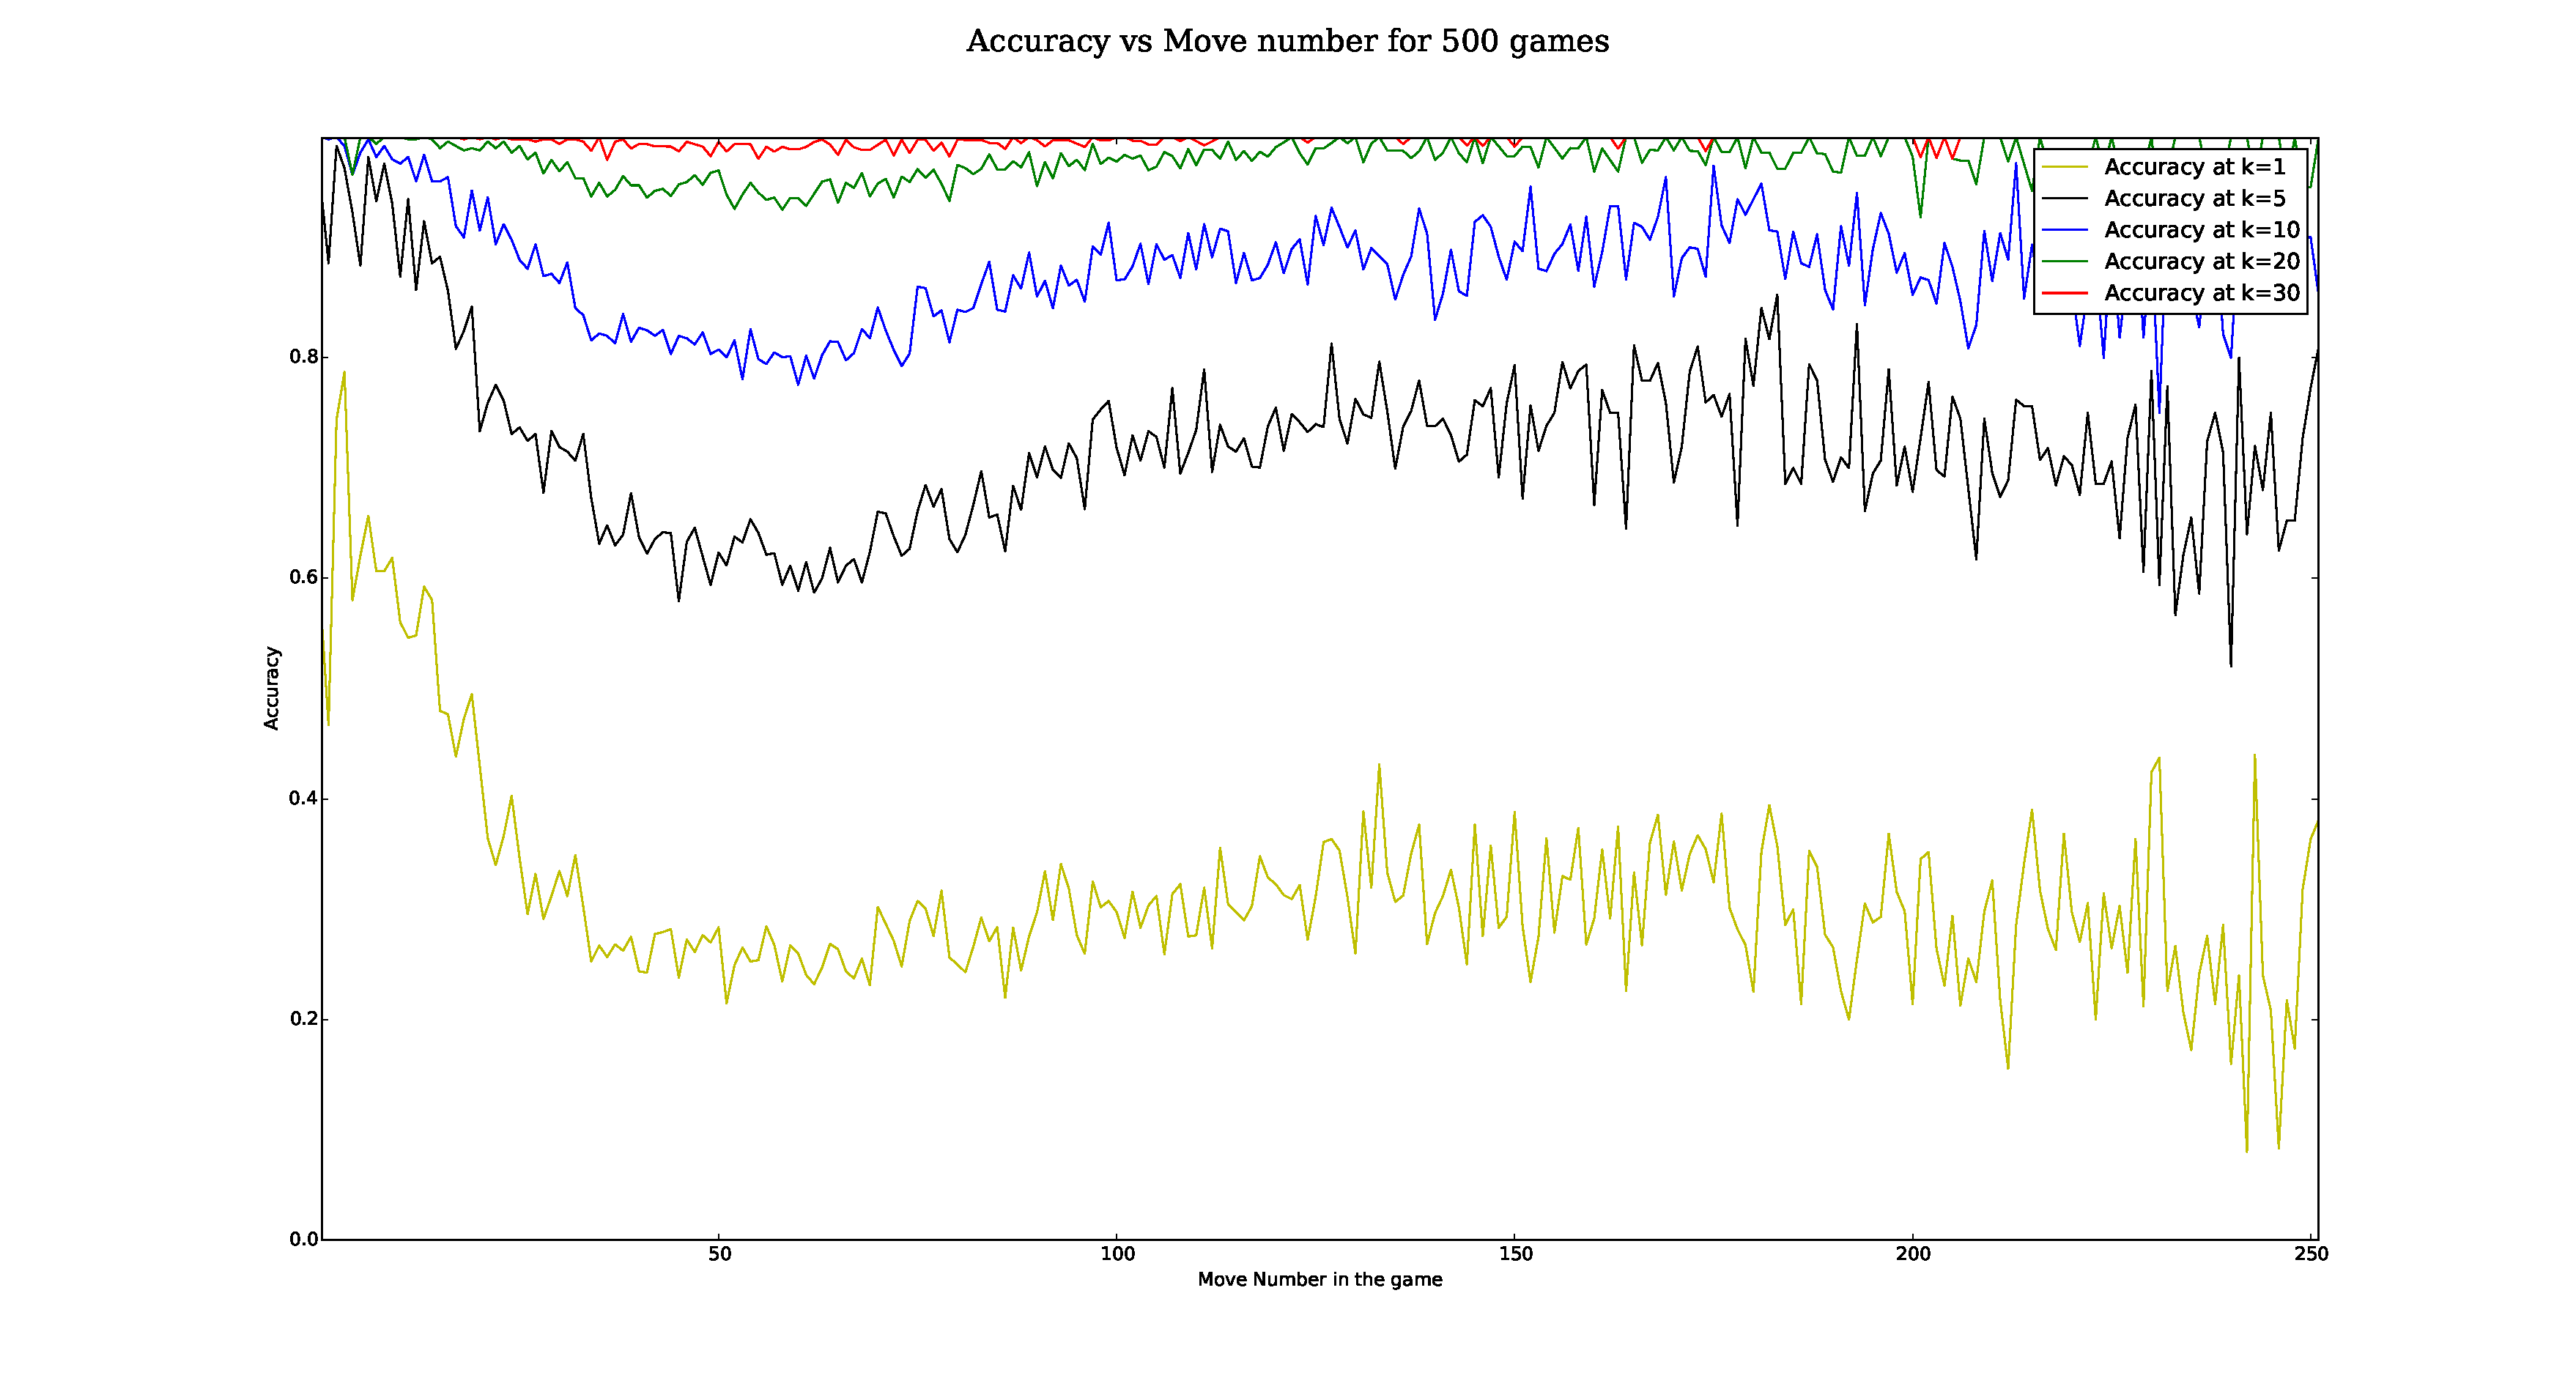
\includegraphics[width=1.5\textwidth,center]{plots/accuracy-move_num2.pdf}
% \caption{Accuracy vs Move number}
% \label{figure:gameplay1}
% \end{figure}
% \begin{figure}
% 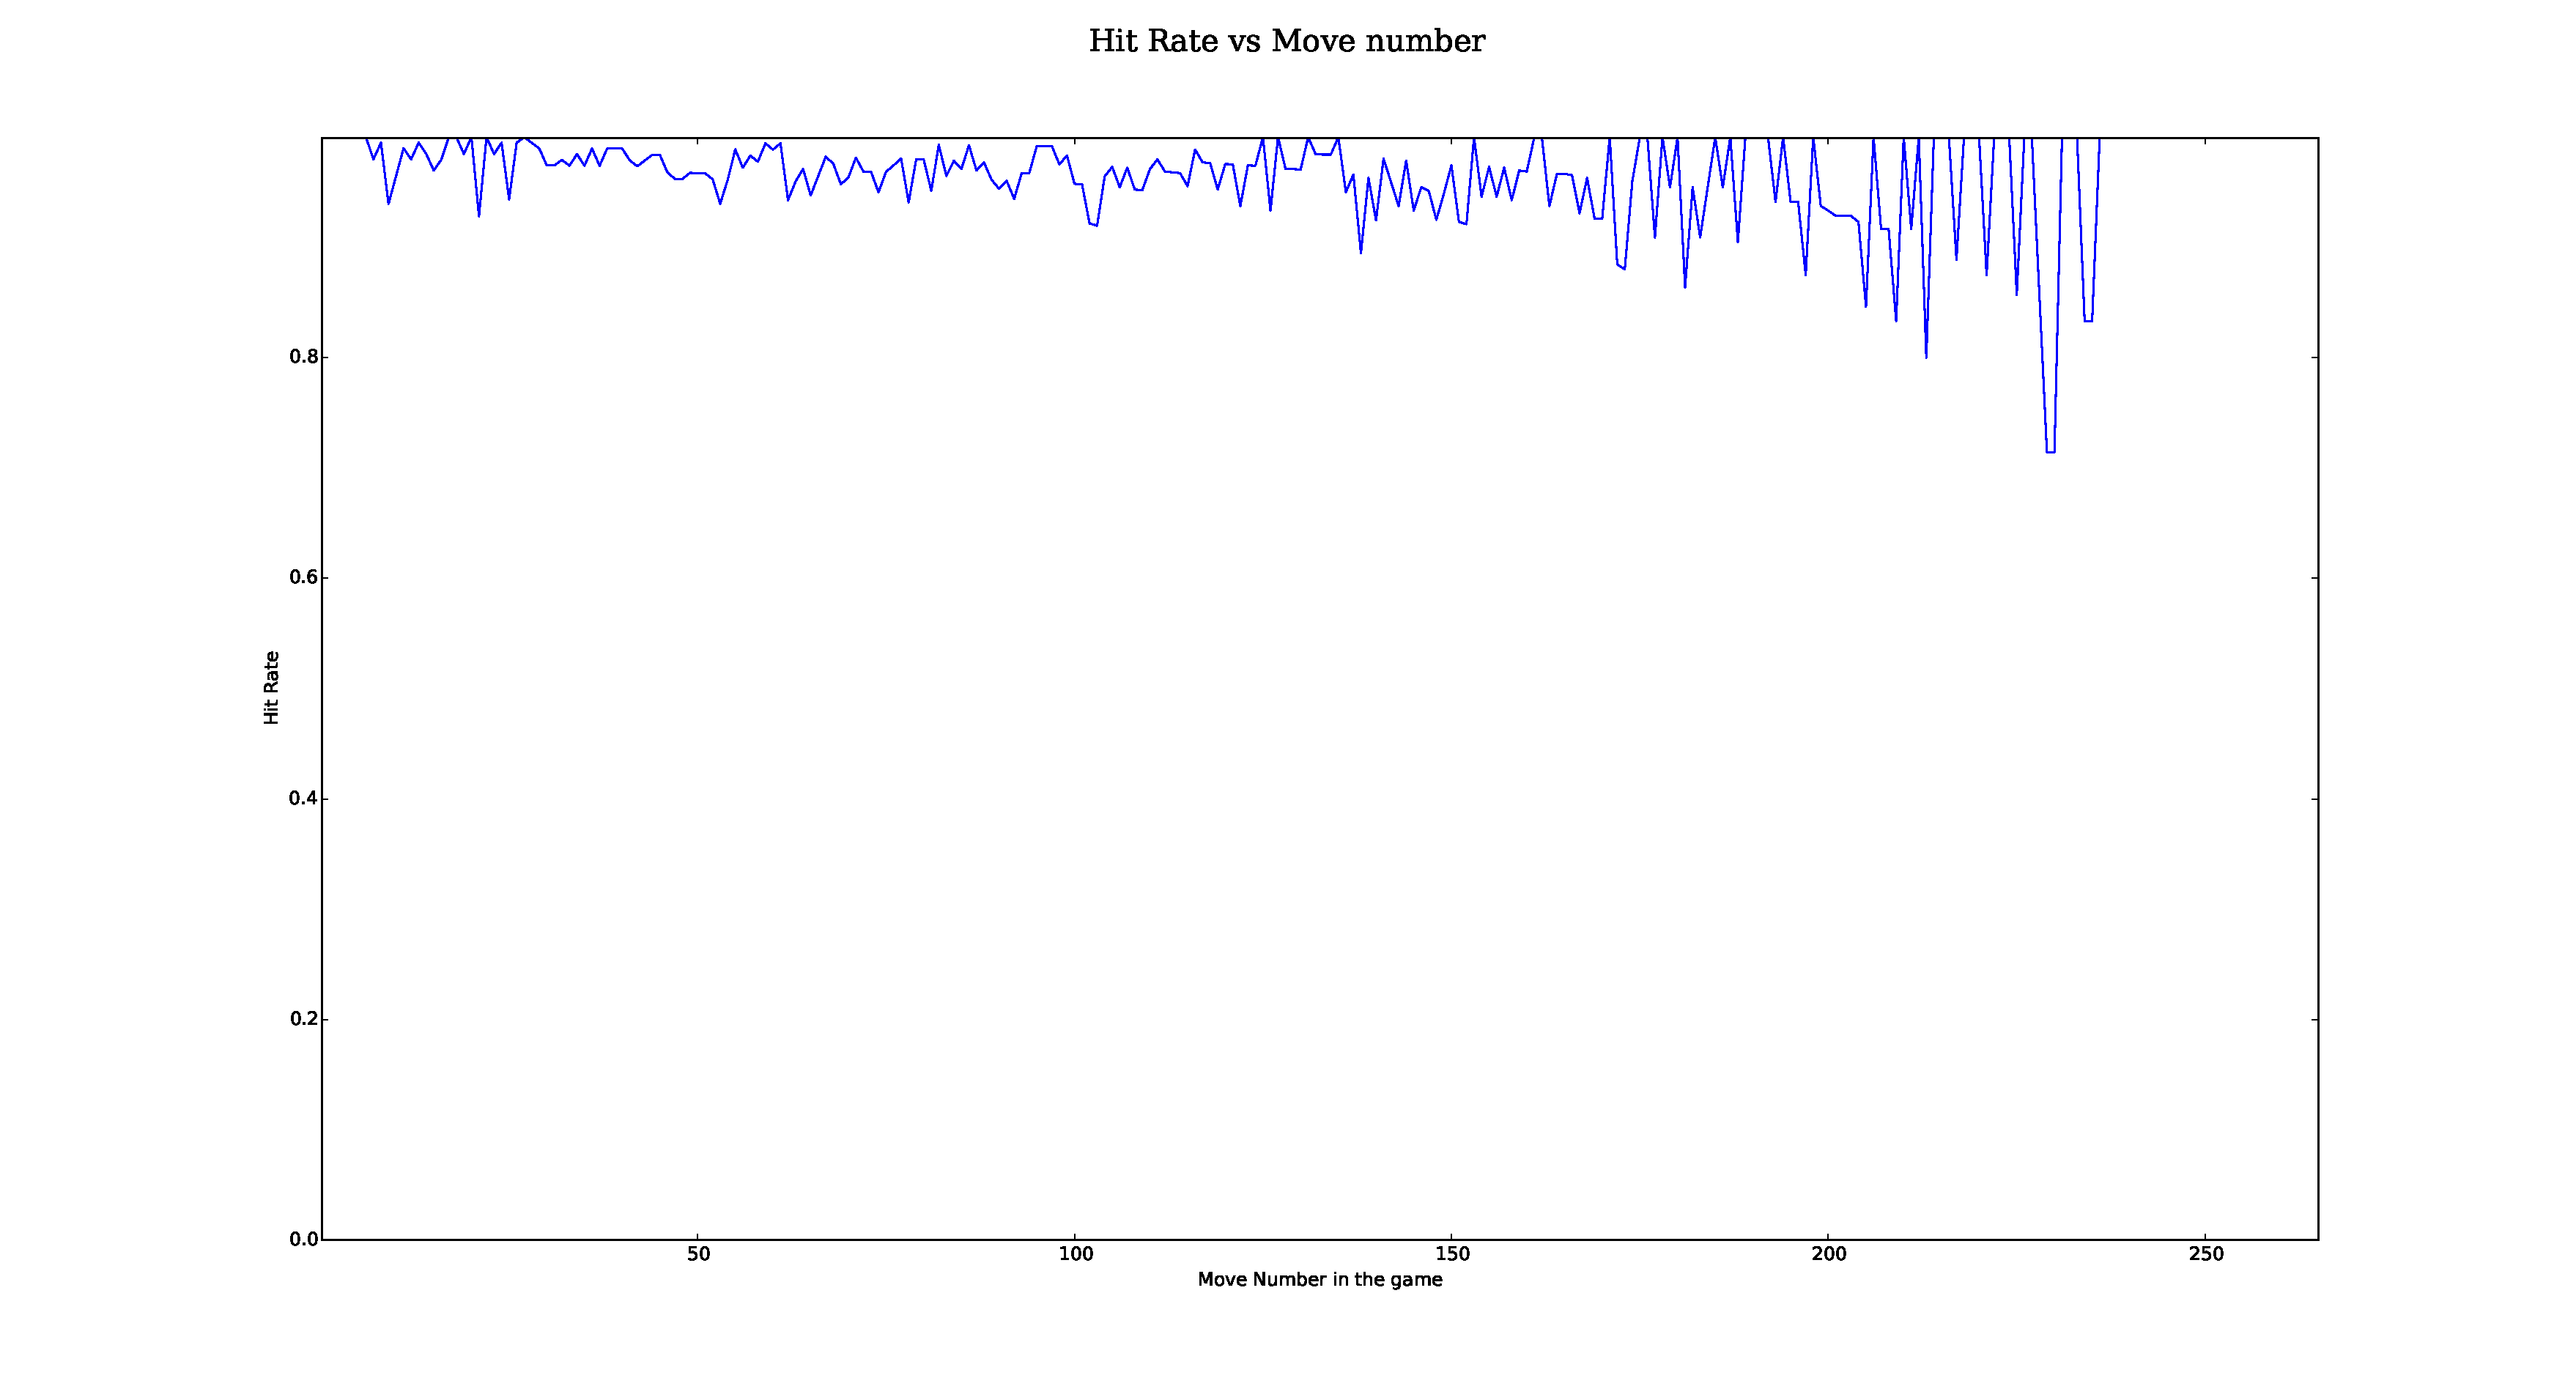
\includegraphics[width=1.5\textwidth,center]{plots/hitrate.pdf}
% \caption{Legal Move rate vs Move Number}
% \label{figure:gameplay2}
% \end{figure}
% \begin{figure}
%   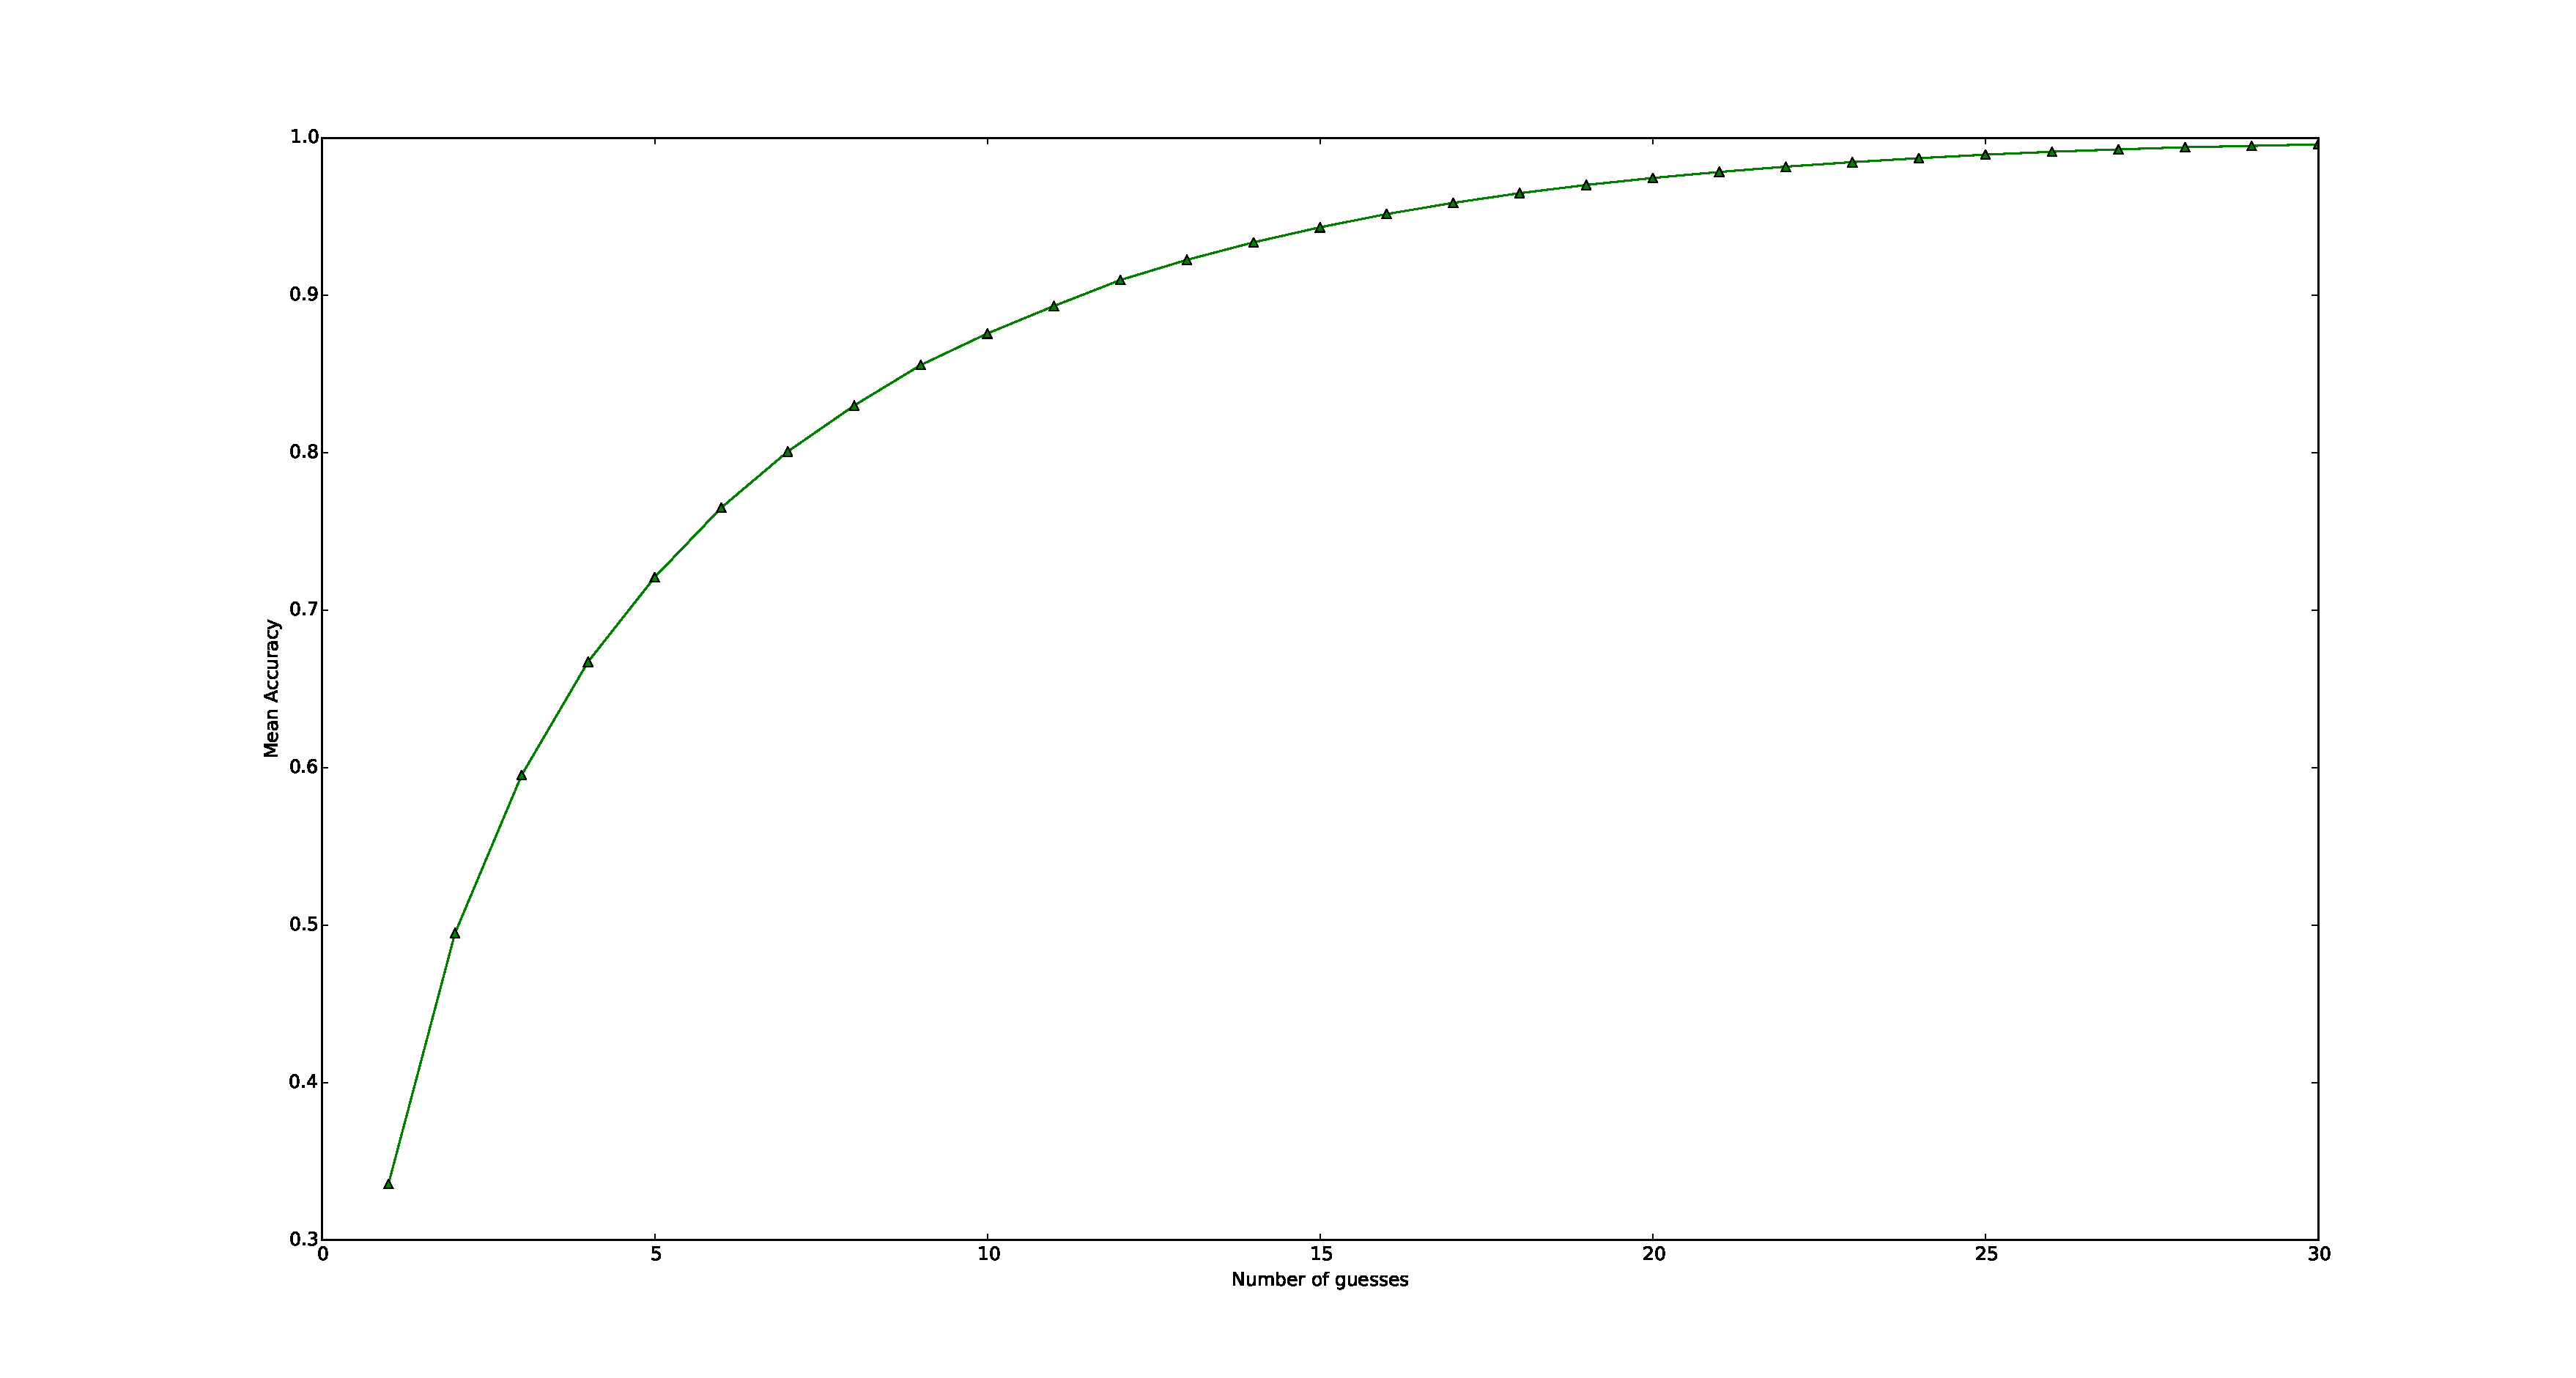
\includegraphics[width=1.5\textwidth,center]{plots/accuracies@k.pdf}
%   \caption{Curves}
%   \label{figure:p}
% \end{figure}%the most important section...Still the worst/no results :(
